\documentclass[12pt, twoside, openany]{report}
\usepackage[dvips]{graphicx,color,rotating}
\usepackage[utf8]{inputenc}
\usepackage{t1enc}
\usepackage{a4wide}
\usepackage{amsfonts}
\usepackage{mathtools}
\usepackage{amsmath}
\usepackage{enumerate}
\usepackage{hyperref}
\usepackage{verbatim}
\usepackage[MeX]{polski}
\usepackage[T1]{fontenc}
\usepackage{geometry}
\geometry{left=25mm,right=25mm,%
bindingoffset=10mm, top=25mm, bottom=25mm}
\usepackage{amssymb, latexsym}
\usepackage{amsthm}
\usepackage{palatino}
\usepackage{array}
\usepackage{pstricks}
\usepackage{textcomp}
\theoremstyle{definition}
\newtheorem{theorem}{Twierdzenie}[section]
\newtheorem{remark}{Uwaga}[section]
\newtheorem{definition}{Definicja}[section]
\newtheorem{alg}{Algorytm}[chapter]
\newtheorem{prz}{Przypadek}[section]
\newtheorem{np}{Przykład}[section]
\newtheorem{lemma}[theorem]{Lemat}
\linespread{1.5}
\newcommand*{\norm}[1]{\left\Vert{#1}\right\Vert}
\newcommand*{\abs}[1]{\left\vert{#1}\right\vert}
\newcommand*{\om}{\omega}

\renewcommand*{\figureautorefname}{Rysunek}
\renewcommand*{\tableautorefname}{Tabela}

\author{Marek Szweda}
\title{Poprawa jakości obrazów cyfrowych poprzez metodę wmalowywania}

\begin{document}

\begin{titlepage}
\pagestyle{empty}

\noindent
\begin{Large}
\begin{table}[t]
\centering
\begin{tabular}[t]{lcr}
 
\includegraphics[width=70pt,height=70pt]{rysunki/PW} & POLITECHNIKA WARSZAWSKA & 
\includegraphics[width=70pt,height=70pt]{rysunki/ele}\\
& WYDZIAŁ ELEKTRYCZNY & \\
\end{tabular}
\end{table}

% \vfill
\begin{center}PRACA DYPLOMOWA MAGISTERSKA\end{center}
%\begin{center}MATEMATYKA\end{center}
\end{Large}
% \vfill
\begin{center}
\Huge
\textbf{Poprawa jakości obrazów cyfrowych poprzez metodę wmalowywania}
\end{center}
% \vfill\vfill
\vfill
\begin{center}
\Large
Autor:\\
\LARGE
Marek Szweda
\end{center}
\vfill
\begin{center}
\Large
Promotor: dr Sławomir Skoneczny
\end{center}
\vfill
\begin{center}
\large
Warszawa, listopad 2018
\end{center}
\newpage
\hfill
\begin{table}[b]
\centering
\begin{tabular}[t]{ccc}
............................................. & \hspace*{100pt} & .............................................\\
podpis promotora & \hspace*{100pt} & podpis autora
\end{tabular}
\end{table}


% \maketitle
\end{titlepage}
\thispagestyle{empty}
\newpage
\pagestyle{headings}
\setcounter{page}{1}
\hyphenation{Syl-ves-tra}
\hyphenation{Syl-ves-ter-a}

\begin{abstract}
Tu będzie jakieś streszczenie
\end{abstract}

%-----------Poczłtek człłci zasadniczej-----------

\chapter{Wprowadzenie}
Poprawa jakości obrazów cyfrowych poprzez metodę wmalowywania w ostatnich czasach stała się jednym z głównych problemów w przetwarzaniu obrazów oraz widzeniu maszynowym. Jest szeroko stosowana w aplikacjach do edycji obrazów, usuwania niechcianych obiektów z obrazów, tekstów, zarysowań, uszkodzeń, poprawy starych zdjęć oraz filmów. Wmalowywanie obrazów definiuje się jako automatyczne wypełnianie braków w obrazie na podstawie otoczenia, w sposób uniemożliwiający obserwatorowi znalezienie pierwotnie wybrakowanych miejsc. Przykłady obrazów poddanych operacji wmalowywania przedstawia \autoref{1_fig1} 
\begin{figure}[!h]
	\centering
	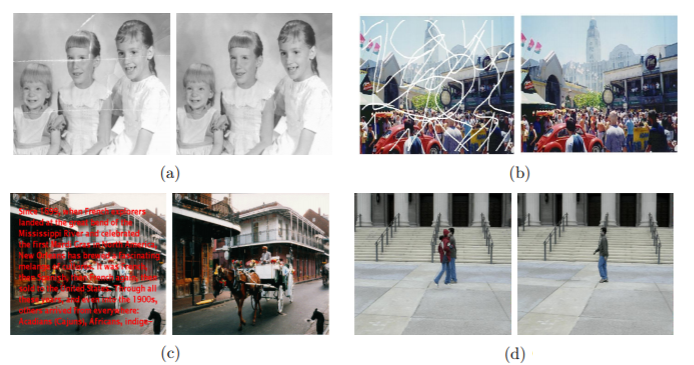
\includegraphics[scale=0.7]{rysunki/fig1}
	\caption{Przykłady obrazów poddanych operacji wmalowywania.}
	\label{1_fig1}
\end{figure}
\par
Obrazy przedstawiono w parze: po lewej obraz wejściowy, po prawej wynikowy obraz poddany operacji wmalowywania. Mogą nimi być uszkodzenia jak w przypadku a oraz b, napisy znajdujące się na obrazie - c, czy też obiekty, którym w konkretnym przypadku d jest postać. Przestrzeń do wmalowywania w obrazie wyznaczana jest manualnie poprzez użytkownika definiującego konkretny obiekt, który powinien według niego zostać usunięty. Program automatycznie nie jest w stanie wyznaczyć części, która powinna zostać przearanżowana.
\par
Techniki wmalowywania znajdują szeroki zakres zastosowań w przetwarzaniu nagrań filmowych, gdzie nieznany region na scenie musi zostać oszacowany w pewien sposób dostarczając spójności wizualnej użytkownikowi. Przykładami mogą być konieczność ukrywania błędów nagrań, strat wynikających z błędów urządzeń nagrywających, czy też usunięcia niepożądanych obiektów, które w trakcie nagrywania pojawiły się w kadrze.
\par
Głównym celem pracy jest osiągniecie algorytmu skutecznie odbudowującego uprzednio zdefiniowaną nieznaną przestrzeń obrazu. W tym celu dokonano przeglądu istniejących algorytmów wmalowywania opartych na rozwiązaniu odpowiednio zdefiniowanych problemów matematycznych. Wyniki badanych zagadnień uzyskiwane są na podstawie danych wejściowych w postaci zdefiniowanych obszarów obrazu otaczających brakujące regiony. Podstawowymi operacjami wykorzystywanymi w bardziej złożonych algorytmach rekonstrukcji są:
\begin{enumerate}
\item
Rozwiązanie cząstkowych równań różniczkowych wyższego rzędu bazujących na kontynuacji tekstur, geometrii, struktur obrazu.
\item
Problem minimalizacji energii o bogatym asortymencie sposobu definicji.
\item
Wyznaczenie podobieństwa pomiędzy obszarami w obrazie za pomocą. wprowadzonej metryki 
\item
Obliczenia przeprowadzane na modelu wariacyjnym
\end{enumerate}
\par
W pracy opisano przedstawione powyżej algorytmy, porównano oraz zaproponowano nowy model uzupełniania brakujących danych. Porównania dokonano na podstawie dwóch najistotniejszych właściwości: szybkości algorytmu oraz obiektywnej oceny poprawności otrzymanego wyniku. Zwrócono także uwagę na różne cechy obrazu, które mogą determinować dobór algorytmu do zadanego problemu. Warto zaznaczyć, iż do tej pory nie została przedstawiona jednoznaczna definicja problemu matematycznego pozwalająca w niezawodny sposób wyznaczyć braki w obrazie niezależnie od jego cech charakterystycznych.
\chapter{Przegląd istniejących algorytmów.}
Pierwszą gałęzią algorytmów zgodnie z rozróżnieniem wprowadzonym w  \cite{SalientStrucTexProp} są metody opierające się na rozwiązaniu równań różniczkowych wyższego rzędu. Wśród nich pojawia się próba przystosowania procesu dyfuzji do wypełniania braków w obrazie (źródła \cite{bertalmio2000image} lub \cite{BertalmioNavierStokes}), dzięki której przy wykorzystaniu zależności z działu mechaniki płynu można dokonać próby kontynuacji informacji z otoczenia w brakujące obszary. Innym sposobem wyznaczenia braków opierającym się na równaniach różniczkowych wyższego rzędu jest próba wprowadzenia problemu minimalizacji energii zdefiniowanej w oparciu o pojęcie wahania funkcji tak jak  \cite{MathematicalModelsforNLTextureInpainting} czy też \cite{ColorTextureInpaintingNLCTVModel}.
\par
Drugą gałęzią algorytmów są metody oparte na uzupełnianiu braków obrazu kawałek po kawałku skopiowanymi częściami istniejącego obrazu z miejsc o najlepszym dopasowaniu w miejsce braku. Pierwszy raz metoda syntezy obrazu kopiowanymi kawałkami została zaproponowana w \cite{efros1999texture}. Kolejność wypełniania braków nie jest obojętna i ma znaczny wpływ na ostateczną spójność obrazu. Jedna z najpopularniejszych metod określania priorytetu została przedstawiona w \cite{criminisi2004region}. Na przestrzeni czasu pojawiło się wiele metod minimalizujących zjawisko niespójności w obrazie takich jak np. \cite{StructurePropagationManual}.
\par
Ostatnią grupą algorytmów jest grupa stanowiąca połączenie powyższych algorytmów. Najprostszym przykładem grupy może być \cite{NavierStokesAndTexturePropagation}, w którym zaproponowano poprzedzenie procesu wmalowywania segmentacją obrazu. Uzyskaną w procesie segmentacji teksturę uzupełnia się metodą najbliższego dopasowania natomiast strukturę uzyskuje na podstawie równań różniczkowych. Kolejnym przykładem może być publikacja \cite{arias2011variational}, w której autorzy proponują nielokalny model wyznaczający nieznany obszar obrazu wykorzystując rachunek wariacyjny, połączony ze zdefiniowaną metryką wyznaczającą odległości pomiędzy rozpatrywanymi skrawkami obrazu.
\par
Większość metod wmalowywania opisanych w literaturze opiera się na algorytmach kontynuujących strukturę, geometrię bądź teksturę obrazu. Modele bazujące na geometrii i strukturze w uogólnieniu generują efekt uboczny w postaci rozmazanego wynikowego obrazu, bez zachowanych tekstur.
Do algorytmów broniących się przed efektem rozmycia wyniku można zaliczyć takie, w których wyznaczeniu konkretnego miejsca w nieznanym obszarze może towarzyszyć przebadanie całego zbioru punktów niemodyfikowanej części obrazu. Stąd metody kontynuujące tekstury w większości uważa się za metody nielokalne.

\chapter{Równania różniczkowe wyższego rzędu.}
\section{Rozwiązanie równania Naviera-Stokesa }
W celu dokładnego nakreślenia idei wmalowywania w oparciu o równanie Naviera-Stokesa należy rozważyć poniższe równanie przepływu cieczy Newtonowskiej:
\begin{equation}
V\nabla V\mathrm{+}\frac{dV}{dt}\mathrm{=-}\frac{\mathrm{1}}{q}\nabla p\mathrm{+}F\mathrm{+}\nu {\nabla }^{\mathrm{2}}V
\label{NavierStokesEquation}
\end{equation}
\begin{equation}
\mathrm{V=\ (-}\frac{\mathrm{\partial }\mathrm{\Psi }}{\mathrm{\partial }\mathrm{y}},\frac{\mathrm{\partial }\mathrm{\Psi }}{\mathrm{\partial }\mathrm{x}}\mathrm{)}
\label{LiquidVelociy}
\end{equation}
gdzie $V$ oznacza prędkość lokalną, $t$ chwilę czasu, $q$ gęstość lokalną, $p$ ciśnienie lokalne, $F$ siłę zewnętrzną działającą lokalnie na ciecz, $\nu$ lepkość kinematyczną lokalną, a $\mathit{\Psi}$ linię prądu. Człon $V\nabla V$ odpowiada konwekcji lokalnego pędu wraz z ruchem cieczy, $\frac{1}{q}\nabla p$ wpływowi sił ciśnieniowych na zmianę pędu (kompensuje niezerową konwekcję),  $F$ sile zewnętrznej działającej na ciecz (np. grawitację) oraz $\nu {\nabla }^2V\ $ dyssypacji pędu cieczy od tarcia pomiędzy cząstkami. Traktując płyn jako nieściśliwy ($q\textrm{?}\infty $)  oraz pomijając działanie sił zewnętrznych ($F=0$)  równanie można uprościć do postaci:
\begin{equation}
 V\nabla V+\frac{dV}{dt}=\nu {\nabla }^2V
\label{NavierStokesEquationShort}
\end{equation}
Zgodnie z \cite{StreamfuntionVorticityForm} dokonując obustronnej rotacji równania otrzymujemy równanie w zależności od wirowości:
\begin{equation}
V\nabla \omega \mathrm{+}\frac{d\omega }{dt}\mathrm{=}\nu {\nabla }^{\mathrm{2}}V
\label{NavierStokesEquationVorticity}
\end{equation}
gdzie wirowość określa się wzorem:
\begin{equation}
\omega =\nabla \times V
\label{Vorticity}
\end{equation}
Zgodnie z \cite{ebrahimi2012navier} niech $I$ reprezentuje obraz cyfrowy będący macierzą o rozmiarze$m \mathrm{\times} n$. Wtedy $I_{i,j}$ zawiera wartość dodatnią całkowitą z przedziału od 0 do 255, stanowiącą informację o poziomie jasności danego piksela z obrazu. Wartość 0 opowiada odcieniu czarnemu, natomiast 255 odcieniu czystemu białemu. Niech D stanowi zbiór indeksów $(i,j)\ \in \ \left\{1,2\dots ,m\right\} \mathrm{\times}$ $\left\{1,2\dots ,n\right\}$. Obraz $I$ wtedy można traktować jako funkcję $I:D\to R$.
\par
W 2000 roku Bertalmio w \cite{BertalmioNavierStokes} wprowadza analogię pomiędzy wirowością a smukłością obrazu. Dokładniej przedstawia to \autoref{tab1}:
\begin{table}[!h]
	\centering
	\begin{tabular}{|cc|c|}
	\hline \hline

		& Navier-Stokes
		& Wmalowywanie w obrazie\\ \hline
		
		& Linia prądu $\ \mathit{\Psi}$ &  Jasność obrazu $I$ \\ \hline
	
		& Prędkość płynu $V = {\mathrm{\nabla }}^{\bot }\mathit{\Psi} = [u, v]$  & Prędkość płynu $V$ = ${\mathrm{\nabla }}^{\bot }I = [u, v]$ \\ \hline
		& Wirowość $\omega =\ {\mathrm{\nabla }}^2\mathit{\Psi}$ & Smukłość $\omega =\ {\mathrm{\nabla }}^2I$ \\ \hline
		
		& Lepkość płynu $\nu $ & Parametr dyfuzji anizotropowej $\nu $ \\
	\hline
	\end{tabular}
	\caption{Mapowanie zmiennych w zagadnieniu wmalowywnia obrazu.}
	\label{tab1}
\end{table}
gdzie ${\nabla }^{\bot }=(\frac{\partial }{\partial y},\frac{\partial }{\partial x})$.
Niech $\mathit{\Omega}\subset D$ stanowi wypełniany obszar obrazu (maskę). W wyniku rozwiązania dyskretnego równania Naviera-Stokesa w przestrzeni maski z warunkami brzegowymi zdefiniowanymi jako jasność pikseli sąsiadujących z obszarem maski uzyskuje się kontynuację linii o podobnej jasności (izolinii) w głąb odrestaurowywanego obszaru zgodnie z \autoref{3_fig1}.  Matematycznie kierunek izolinii jasności obrazu wyznacza ${\nabla }^{\bot }I$. W oparciu o \autoref{tab1} oraz \eqref{NavierStokesEquationVorticity} zagadnienia wmalowywania można sformułować jako problem stabilnego rozwiązania poniższego równania różniczkowego:
\begin{equation}
{\mathrm{(}\mathrm{\nabla }}^{\mathrm{\bot }}I\mathrm{)}\mathrm{\cdot }\nabla {\mathrm{(}\mathrm{\nabla }}^{\mathrm{2}}I\mathrm{)+}\frac{d{\mathrm{(}\mathrm{\nabla }}^{\mathrm{2}}I\mathrm{)}}{dt}\mathrm{=}\nu \mathrm{\nabla }\mathrm{(}g\mathrm{(}\nabla {\mathrm{(}\mathrm{\nabla }}^{\mathrm{2}}I\mathrm{))}\nabla {\mathrm{(}\mathrm{\nabla }}^{\mathrm{2}}I\mathrm{))} 
\label{NavierStokesInpainting}
\end{equation}
\begin{figure}[!h]
	\centering
	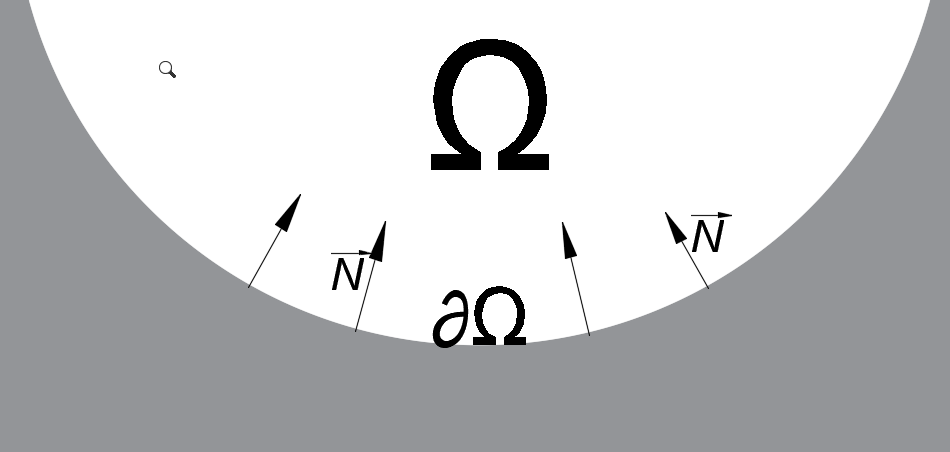
\includegraphics[scale=1]{rysunki/3_fig1}
	\caption{Propagacja jasności obrazu wgłąb nieznanego obszaru.}
	\label{3_fig1}
\end{figure}
W równaniu \eqref{NavierStokesInpainting} człon odpowiedzialny za tarcie pomiędzy cząstkami płynu $\nu {\nabla }^2V\ $ został zastąpiony dyfuzją anizotropową, która w kontekście przetwarzania obrazów pierwszy raz wprowadzona została przez Perona i Malika w 1987 roku. Dyfuzja anizotropowa ma znaczny wpływ na zachowanie krawędzi obrazu oraz poprawę jego ostrości. Za dyfuzję anizotropową odpowiada współczynnik $g$, który przedstawiany jest w różnych postaciach funkcji przewodności. W pracy wykorzystana zostanie postać:
\begin{equation}
g\left(s\right)=\frac{1}{1+\alpha \left|s\right|}
\end{equation}
gdzie $\alpha\ $, $K$ uprzednio zdefiniowane parametry dyfuzji (stałe), ${\mathrm{\nabla }}^{\bot }=({-\partial }_y,{\partial }_x)$. 
Dyskretne rozwiązanie równania \eqref{NavierStokesInpainting} jest analogiczne do dyskretnego rozwiązania przepływu płynu w przestrzeni $2D$. W tym celu należy wprowadzić chwile w czasie $t=n\bullet \Delta t$, gdzie $n=\left\{1,2,3,\dots ,N\right\}$, $\Delta t$ wartość przyrostu czasu pomiędzy dyskretnymi chwilami $n$ i $n+1$, $N$ moment osiągnięcia stanu ustalonego, matematycznie przedstawianego jako:
\begin{equation}
\frac{\partial I}{\partial t}\mathrm{+}{\mathrm{\nabla }}^{\mathrm{\bot }}I\mathrm{\nabla }\mathrm{\Delta }I\mathrm{\ }\mathrm{\cong }\mathrm{0}
\label{NavierStokesStability}
\end{equation}
Warto zauważyć, że człon ${\mathrm{\nabla }}^{\bot }I$ w równaniu \eqref{NavierStokesStability} odpowiada kierunkowi rozchodzenia się punktów o podobnej jasności, natomiast $\mathrm{\nabla }\Delta I$ to kierunek największej zmiany smukłości obrazu. Jeśli wektory są do siebie prostopadłe (do czego zbiega algorytm) iloczyn skalarny wynosi 0. 
W celu dokładnej analizy dyskretyzacji równanie \eqref{NavierStokesEquationVorticity} zostanie rozdzielone na dwa podrównania:
\begin{equation}
\frac{d{\mathrm{(}\mathrm{\nabla }}^2I)}{dt}=-{\mathrm{(}\mathrm{\nabla }}^{\bot }I)\cdot \nabla {\mathrm{(}\mathrm{\nabla }}^2I)+\left\{ad\right\}
\label{NavierDiffAdv}
\end{equation}
oraz
\begin{equation}
ad=\nu \mathrm{\nabla }(g(\nabla {\mathrm{(}\mathrm{\nabla }}^2I))\nabla {\mathrm{(}\mathrm{\nabla }}^2I))
\label{NavierAdv}
\end{equation}
Rozwiązanie powyższych równań dokonywane będzie na siatce obliczeniowej typu Eulera, a wszystkie wartości wyznaczanych zmiennych będą znajdować się w centrach komórki zdefiniowanej jako konkretny piksel obrazu, zgodnie z \autoref{3_fig1} 
\begin{figure}[!h]
	\centering
	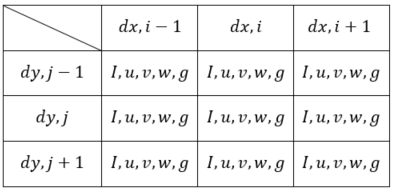
\includegraphics[scale=0.7]{rysunki/fig2}
	\caption{Przykłady obrazów poddanych operacji wmalowywania.}
	\label{3_fig2}
\end{figure}
Równanie \eqref{NavierDiffAdv} to równanie różniczkowe cząstkowe typu parabolicznego. Zgodnie z teorią równanie można rozwiązać metodą różnic skończonych schematem centralnym bądź schematem do przodu. W przypadku równania parabolicznego oba schematy dostarczają stabilnego rozwiązania. W celu ułatwienia dalszych rozważań wprowadzono funkcję $f$ określoną w centrach siatki, z przypisami dolnymi wskazującymi na konkretne miejsce w siatce. Korzystając z rozwinięcia w szereg Taylora gradient funkcji $f$ w punkcie $(i,j)$  można przybliżyć następującym wzorem:
\begin{equation}
\nabla f_{i,j}=\left|\ {\frac{\partial f}{\partial x}|}_{i,j,}{\frac{\partial f}{\partial y}|}_{i,j}\right|
\label{gradF}
\end{equation}
gdzie:
\begin{equation}
{\frac{\partial f}{\partial x}|}_{i,j}=\frac{f_{i+1,j}+f_{i-1,j}}{2\Delta x}
\label{dfdx}
\end{equation}
Analogicznie:
\begin{equation}
{\frac{\partial f}{\partial y}|}_{i,j}=\frac{f_{i,j+1}+f_{i,j-1}}{2\Delta y}
\label{dfdy}
\end{equation}
Na podstawie powyższych wzorów składowe wektora ${\mathrm{\nabla }}^{\bot }I$, czyli kierunku, w którym należy propagować smukłość obrazu ${\mathrm{\nabla }}^2I$ wyznacza się z zależności:
\begin{equation}
u_{i,j}=\frac{I_{i,j+1}+I_{i,j-1}}{2\Delta y} 
\label{u}
\end{equation}
Oraz
\begin{equation}
 v_{i,j}=-\frac{I_{i+1,j}+I_{i-1,j}}{2\Delta x}
\label{v}
\end{equation}
Gdzie:
\begin{equation}\\
{\mathrm{\nabla }}^{\bot }I=|-u,v|
\label{gradI}
\end{equation}
Stosując pięciopunktowy analog różnicowy w metodzie skończonych różnic operator Laplace’a dla przyjętej siatki Eulera można przybliżyć wzorem (przy założeniu $\Delta x=\ \Delta y$):
\begin{align}
\begin{aligned}
{\mathrm{\nabla }}^2f_{i,j} &= \Delta f_{i,j} \\[1ex]
&={\frac{{\partial }^2f}{\partial x^2}|}_{i,j}+{\frac{{\partial }^2f}{\partial y^2}|}_{i,j} \\
&=\frac{f_{i+1,j+1}+f_{i-1,j+1}+f_{i+1,j-1}+f_{i-1,j-1}-4f_{i,j}}{\Delta x^2}\ 
\end{aligned}
\label{LaplaceOpr}
\end{align}
Korzystając z wyznaczonych powyżej zależności na wartości $u$ oraz $v$ wartość smukłości obrazu $\omega =\ {\mathrm{\nabla }}^2I$ można przedstawić w postaci: 
\begin{equation}
\Delta {I|}_{i,j}=\ {\frac{\partial v}{\partial x}|}_{i,j,}-\ {\frac{\partial u}{\partial y}|}_{i,j}
\label{discreteVorticity}
\end{equation}
Podobnie jak w przypadku liczenia pochodnej w przestrzeni powierzchni (obrazu) pierwszą pochodną w przestrzeni czasu przybliża się rozwinięciem w szereg Taylora. Niech przypis górny oznacza konkretną chwilę w czasie. Wtedy wartość pochodnej wynosi:
\begin{equation}
\ {{\frac{\partial f}{\partial t}|}^n_{i,j}=\ \frac{f^{n+1}_{i,j}-\ f^n_{i,j}}{\Delta t}}
\label{dfdt}
\end{equation}
Ostatecznie rozwiązanie dyskretnego równania parabolicznego \eqref{NavierDiffAdv} , gdzie $\Delta x= \Delta y=h$, z wykorzystaniem schematu centralnego ma postać:
\begin{align}
{\omega }^{n+1}_{i,j} &= {\omega }^n_{i,j}+\Delta t\biggl[
-\left(\frac{I_{i,j+1}+I_{i,j-1}}{2h}\right)\left(\frac{{\omega }_{i+1,j}
+{\omega }_{i-1,j}}{2h}\right)  \notag\\ 
&\qquad+ \left(\frac{I_{i+1,j}+I_{i-1,j}}{2h}\right)\left(\frac{{\omega }_{i,j+1}+{\omega }_{i,j-1}}{2h}\right)+{\left\{ad\right\}}_{i,j} \biggr]
\label{NavierDiffAdvCen}
\end{align}
Rozwiązanie równania \eqref{NavierDiffAdv} można przedstawić również w drugiej postaci wykorzystującej schemat „do przodu”, charakteryzujący się wyznaczaniem wartości pochodnej wirowości w zależności od wyznaczonego kierunku ${\mathrm{(}\mathrm{\nabla }}^{\bot }I)$.  Wtedy równanie \eqref{NavierDiffAdvCen} przyjmuje postać:
\begin{align}
{\omega }^{n+1}_{i,j} &= {\omega }^n_{i,j}+\Delta t\biggl[
-\left(\frac{I_{i,j+1}+I_{i,j-1}}{2h}\right)\left(\frac{{\omega }_{i+sgn\left(u^n\right),j}+{\omega }_{i,j}}{2h}\right)  \notag\\ 
&\qquad+ \left(\frac{I_{i+1,j}+I_{i-1,j}}{2h}\right)\left(\frac{{\omega }_{i,j+sgn(u^n)}+{\omega }_{i,j}}{2h}\right)+{\left\{ad\right\}}_{i,j} \biggr]
\label{NavierDiffAdvFor}
\end{align}
\par
Rozwiązanie równania \eqref{NavierAdv}, w którym zastąpiono postać zwykłej dyfuzji $\nu {\nabla }^2V$ wymaga uważniejszego potraktowania ze względu na większą podatność na niestabilność implementowanych metod dyskretyzacji. Równanie można przedstawić w postaci dywergencji pola wektorowego uzyskanego w wyniku gradientu wirowości z uwzględnionym współczynnikiem dyfuzji anizotropowej:
\begin{align}
\begin{aligned}
\left\{ad\right\} 
&= \nu \mathrm{\nabla }(g(\nabla {\mathrm{(}\mathrm{\nabla }}^2I))\nabla {\mathrm{(}\mathrm{\nabla }}^2I) \\[1ex]
&= \nu \mathrm{\nabla }\mathrm{\cdot}(g(|\nabla \omega |)\nabla \omega )   \\[1ex]
&= {\partial }_x\left(g\left(\left|\nabla \omega \right|\right){\partial }_x\omega \right)+{\partial }_y\left(g\left(\left|\nabla \omega \right|\right){\partial }_y\omega \right)
\end{aligned}
\label{Anisotropic}
\end{align}
\eqref{Anisotropic}
gdzie: ${\partial }_x=\frac{\partial }{\partial x}$ oraz analogicznie: ${\partial }_y=\frac{\partial }{\partial y}$.
Zgodnie z \cite{ebrahimi2012navier} powyższe równanie można rozwiązać w poniższych krokach:
Korzystając z zależności \eqref{dfdx} i \eqref{dfdy} wyznaczyć wartości $({\frac{d\omega }{dx})}_{i,j}$ oraz $({\frac{d\omega }{dy})}_{i,j}$
Na podstawie wartości z punktu 1 obliczyć moduł wektora dla przestrzeni Euklidesowej:
\begin{equation}
{\left|\mathrm{\nabla }\omega \right|}_{i,j}=\ \sqrt{\mathrm{\ }({\frac{\partial \omega }{\partial x})}^2_{i,j}+{\left(\frac{\partial \omega }{\partial y}\right)}^2_{i,j}\ }\
\label{magnitudedw}
\end{equation}
Na podstawie wartości z punktu 2 wyznaczyć wartość $$\ g{\left({\left|\mathrm{\nabla }\omega \right|}_{i,j}\right)}_{i,j}$$ wykorzystując \eqref{NavierStokesInpainting}. Korzystając z wartości wyznaczonych powyżej oraz ponownie z zależności \eqref{dfdx} i \eqref{dfdy} obliczyć:
\begin{align}
{\left\{ad\right\}}_{i,j} &= {\left({\partial }_x\left(g{\left({\left|\mathrm{\nabla }\omega \right|}_{i,j}\right)}_{i,j}{\left({\frac{d\omega }{dx})}_{i,j}\right)}_{i,j}\right)\right)}_{i,j} \notag \\[1ex]
&+ {\left({\partial }_y\left(g{\left({\left|\mathrm{\nabla }\omega \right|}_{i,j}\right)}_{i,j}{\left({\frac{d\omega }{dx})}_{i,j}\right)}_{i,j}\right)\right)}_{i,j}
\label{discreteAnisotropic}
\end{align}
\par
Innym sposobem dyskretyzacji równania \eqref{NavierAdv} może być metoda przedstawiona w \cite{van2005algorithms}, wykorzystująca asymetryczny schemat liczenia pierwszej pochodnej funkcji. Pierwsze pochodne asymetryczne lewe przyjmują postać:
\begin{equation}
{\frac{{\partial }^-f}{\partial x}|}_{i,j}=\frac{f_{i,j}+f_{i-1,j}}{\Delta x}
\label{leftdfdx}
\end{equation}
\begin{equation}
{\frac{{\partial }^-f}{\partial y}|}_{i,j}=\frac{f_{i,j}+f_{i,j-1}}{\Delta y}
\label{leftdfdy}
\end{equation}
Analogicznie prawe:
\begin{equation}
{\frac{{\partial }^+f}{\partial x}|}_{i,j}=\frac{f_{i+1,j}+f_{i,j}}{\Delta x} 
\label{rightdfdx}
\end{equation}
\begin{equation}
{\frac{{\partial }^+f}{\partial y}|}_{i,j}=\frac{f_{i,j+1}+f_{i,j}}{\Delta y}
\label{rightdfdy}
\end{equation}
Następnie powyższe zależności znajdują zastosowanie w wyznaczeniu członów\\ ${\partial }_y\left(g\left(\left|\nabla \omega \right|\right){\partial }_y\omega \right)$ oraz ${\partial }_x\left(g\left(\left|\nabla \omega \right|\right){\partial }_x\omega \right)+{\partial }_y$. Stosując naprzemiennie schemat lewy z prawym do liczenia wartości pochodnych wewnętrznych i zewnętrznych w wyniku otrzymuje się ogólny schemat centralny. Stosując powyższe ostatecznie równanie \eqref{NavierAdv} można przedstawić w następującej postaci dyskretnej:
\begin{align}
\begin{aligned}
{\left\{ad\right\}}_{i,j}
&= \frac{1}{2}\biggl[\left(g_{i,j}+g_{i+1,j}\right)\left({\omega }_{i+1,j}-{\omega }_{i,j}\right) \\[1ex]
&- \left(g_{i-1,j}+g_{i,j}\right)\left({\omega }_{i,j}-{\omega }_{i-1,j}\right)   \\[1ex]
&+ \left(g_{i,j}+g_{i,j+1}\right)\left({\omega }_{i,j+1}-{\omega }_{i,j}\right) \\[1ex]
&- \left(g_{i,j-1}+g_{i,j}\right)\left({\omega }_{i,j}-{\omega }_{i,j-1}\right)\biggl]
\end{aligned}
\label{discreteAnisotropic2}
\end{align}
Należy zauważyć, iż do wyznaczenia wartości $u$, $v$ oraz ${\mathrm{\nabla }}^2I$ wykorzystywanych do obliczeń \eqref{NavierDiffAdv} i \eqref{NavierAdv} w każdej kolejnej chwili czasu $n$, konieczna jest znajomość obrazu $I^n$. W związku z tym równolegle do równania \eqref{Vorticity} należy rozwiązywać poniższe niejednorodne równanie różniczkowe cząstkowe liniowe drugiego rzędu.
\begin{equation}
\Delta I^n={\omega }^n
\label{Poisson}
\end{equation}
Dla przestrzeni dwuwymiarowej równanie przyjmuje postać:
\begin{equation}
\frac{{\partial }^2I}{\partial x^2}+\frac{{\partial }^2I}{\partial y^2}=\ \omega
\label{Poisson2D}
\end{equation}
W celu przybliżenia drugiej pochodnej funkcji $f$ w punkcie $(i,j)$ należy rozwinąć funkcję $f$ w dwa szeregi Taylora względem punktu $(i+1,j)$ oraz $(i-1,j)$. Po rozwiązaniu sumy dwóch rozwinięć względem $\frac{{\partial }^2f}{\partial x^2}$ otrzymuje się poniższy sposób dyskretyzacji drugiej pochodnej:
\begin{equation}
{\frac{{\partial }^2f}{\partial x^2}\mathrm{|}}_{i,j}\mathrm{=}\frac{f_{i+1,j}-2f_{i,j}+f_{i-1,j}}{\Delta x^2}
\label{d2fdx2}
\end{equation}
Analogicznie:
\begin{equation}
{\frac{{\partial }^2f}{\partial y^2}\mathrm{|}}_{i,j}\mathrm{=}\frac{f_{i,j+1}-2f_{i,j}+f_{i,j-1}}{\Delta y^2}
\label{d2fdy2}
\end{equation}
Korzystając z \eqref{d2fdx2} oraz \eqref{d2fdy2} równanie \eqref{Poisson} w punkcie $(i,j)$ przyjmuje postać pięciopunktowego analogu różnicowego operatora $\Delta $ ($\Delta x=\ \Delta y=h)$:
\begin{equation}
I_{i+1,j}+I_{i-1,j}+I_{i,j+1}+I_{i,j-1}-4I_{i,j}=h^2{\omega }_{i,j}
\label{Laplace}
\end{equation}
Na podstawie równania \eqref{Laplace} można stworzyć równanie macierzowe postaci $Ax=B$, gdzie $x$ reprezentuje obraz $I$, $B$ smukłość obrazu, natomiast $A$ to macierz charakterystyczna współczynników. Istnieje wiele metod rozwiązywania równań Poissona takich jak metoda Jacobiego czy Gaussa-Seidla.  Wystarczającą wydajność i szybkość działania w celach rozwiązania równania można uzyskać stosując metodę SOR – sukcesywnej nadrelaksacji. Dyskretyzacja równania wygląda następująco:
\begin{align}
\begin{aligned}
I^{n+1}_{i,j}
&= \left(1-\ \beta \right)I^n_{i,j}+\beta \cdot \frac{1}{2}{\left(\frac{1}{\Delta x^2}+\frac{1}{\Delta y^2}\right)}^{-1}\\[1ex]
&\cdot \left[\frac{1}{\Delta x^2}{(I}^n_{i+1,j}+I^{n+1}_{i-1,j})+\frac{1}{\Delta y^2}{(I}^n_{i,j+1}+I^{n+1}_{i,j-1})+{\omega }^n_{i,j}\right]
\end{aligned}
\label{DiscreteSOR}
\end{align}
Metoda w swoim równaniu przyjmuje parametr wagowy $\beta$ odpowiadający za zbieżność algorytmu. Dobór nie jest losowy i zawiera się w przedziale $(0,2)$. Zgodnie z literaturą parametr ten powinno przyjmować się zgodnie z zależnością:
\begin{equation}
{\omega }_{opt}=2{\left(1+\frac{\pi }{N}\right)}^{-1}
\label{BetaChoose}
\end{equation}
gdzie $N$ to liczba kolumn przyjętej siatki obliczeniowej. 
\par
Operacje wmalowywania bardzo często wykonywane są w punktach maski tworzących nieregularne kształty, mogących znajdować się w różnych częściach obrazu. Stąd powyżej przedstawiony schemat obliczeń wykonywany jest dla wszystkich pikseli obrazu. Po każdej iteracji uzyskane wartości $I^{n+1}$ w znanych punktach przepisywane są z oryginalnego obrazu $I_{o}$, zgodnie z zależnością poniżej.
\begin{equation}
I^{n+1}(D/\mathrm{\Omega }\mathrm{)\ }\ ={\ I}_o(D/\mathrm{\Omega }\mathrm{)}
\label{retrieveMask}
\end{equation}
\par
Podsumowując w celu wyznaczenia niewiadomych wartości obrazu w punktach zdefiniowanych przez maskę należy powtarzać następujące iteracje do uzyskania stanu ustalonego:
\begin{enumerate}
\item
Rozwiązać równanie \eqref{discreteAnisotropic} 
\item
Na podstawie równania \eqref{NavierDiffAdvCen} zamiennie z \eqref{NavierDiffAdvFor} wyznaczyć wartości $\omega_{i,j}^{n+1}$ dla każdego punktu $(i,j)$ 
\item
Korzystając z \eqref{DiscreteSOR} wyznaczyć jasność każdego piksela $I_{i,j}^{n+1}$.
\item
Do uzyskanego obrazu w punkcie 3 przepisać znane wartości z obrazu oryginalnego
\end{enumerate}
Powyższy algorytm przedstawiono dla obrazów w odcieniach szarości. W celu implementacji rozwiązania dla obrazów kolorowych, których funkcję definiuje się jako przekształcenie w pole wektorowe $[R,G,B]$, czyli $I:D\to R^3$  zgodnie z propozycją w \cite{fishelov2006image} można w pierwszym kroku przekształcić do współrzędnych sferycznych $\left[I_{1},I_{2},I_{3} \right]$ korzystając z zależności:
\begin{equation}
{I_{1_{i,j}}=r}_{i,j}=\ \sqrt{R^2_{i,j}+G^2_{i,j}+B^2_{i,j}}
\label{TIone}
\end{equation}
\begin{equation}
I_{2_{i,j}}=\ {\mathrm{sin} {\mathrm{\Theta }}_{i,j}\ }=\ {\mathrm{sin} {{\mathrm{tan}}^{-1} \frac{G_{i,j}}{R_{i,j}}\ }\ } 
\label{TItwo}
\end{equation}
\begin{equation}
I_{3_{i,j}}=\ {\mathrm{sin} {\phi }_{i,j}\ }=\ {\mathrm{sin} {{\mathrm{cos}}^{-1} \frac{B_{i,j}}{r_{i,j}}\ }\ } 
\label{TIthree}
\end{equation}
Następnie dysponując komponentami $I_1$, $I_2$, $I_3$ wyznaczonymi z powyższych zależności, dla każdego z nich oddzielnie należy wykonać wcześniej opisane iteracje. W celu odwrotnego przekształcenia $\left[I_1,I_2,I_3 \right]\to\left[R,G,B\right]$ wystarczy wykonać poniższe obliczenia:
\begin{equation}
 B_{i,j}=\ r_{i,j}{\mathrm{cos} {\mathrm{\Theta }}_{\mathrm{i,j}}\ }{\mathrm{cos} {\phi }_{\mathrm{i,j}}\ }
\label{TInvIone}
\end{equation}
\begin{equation}
R_{i,j}=\ r_{i,j}{\mathrm{cos} {\mathrm{\Theta }}_{\mathrm{i,j}}\ }{\mathrm{sin} {\phi }_{\mathrm{i,j}}\ }
\label{TInvItwo}
\end{equation}
\begin{equation}
G_{i,j}=\ r_{i,j}{\mathrm{sin} {\theta }_{\mathrm{i,j}}\ } 
\label{TInvIthree}
\end{equation}
Operację wmalowywania można wykonać na pierwotnych komponentach $[R,G,B]$ lecz matematyczna transformacja przestrzeni charakteryzuje się lepszymi właściwościami związanymi z postrzeganiem różnicy barw $\delta E$ przez ludzkie oko:
\begin{equation}
\Delta E=\ \sqrt{{\left(\Delta I_1\right)}^2+{\left(\Delta I_2\right)}^2+{\left(\Delta I_3\right)}^2}
\label{deltaE}
\end{equation}
\section{Problem minimalizacji energii}
	Innym sposobem zastosowania równań różniczkowych w procesie wmalowywania obrazu może być może być adaptacja problemu minimalizacji energii. Pojęcie wahania funkcji $TV$ w analizie obrazów pierwszy raz wprowadzone zostało przez Rudin, Osher i Fatemi’ego w \cite{rudin1992nonlinear}, gdzie proponowany model znajduje zastosowanie w usuwaniu szumów z obrazu. Następnie model $TV$ zostaje zaproponowany do wmalowywania obrazu w \cite{MathematicalModelsforNLTextureInpainting} przez Chan i Shen’a. Problem doboru parametrów dla modelu $TV$, właściwości oraz proces dyskretyzacji problemu minimalizacji jest dokładnie przedstawiony w \cite{getreuer2012total}. Algorytm bazujący na lokalnych funkcjonałach $TV$  charakteryzuje się zdolnością do kontynuacji geometrycznych struktur obrazu i krawędzi. Zgodnie z przedstawioną literaturą wadą algorytmu jest brak możliwości propagacji tekstury w nieznany obszar $\Omega$. Warto wspomnieć, iż w przypadku usuwania szumów z obrazów wykorzystanie lokalnych operatorów nie pozwala zachować tekstur. Problem jednoczesnej propagacji geometrii i tekstury można rozwiązać przy zastosowaniu nielokalnego modelu, który zostanie poddany analizie w niniejszej pracy.
	Klasyczny nielokalny model wahania funkcji został intensywnie przebadany dla obrazów w odcieniach szarości. W przypadku obrazów kolorowych jednym z pierwszych zaproponowanych modeli jest model Mumford-Shah dokładnie opisany w \cite{jung2011nonlocal}. Model ten dla każdej z warstw obrazu kolorowego przeprowadza oddzielną analizę, w wyniku prowadząc do niejednorodnego kontrastu kolorów obrazu w przestrzeni wmalowywanej $\Omega$ z jego otoczeniem $D/\mathrm{\Omega}$. Problem uzyskania jednakowego kontrastu rozwiązano poprzez propozycję nowego, szybkiego modelu w \cite{duan2015fast} wprowadzającego zależność pomiędzy wszystkimi warstwami obrazu kolorowego. W celu analizy nowego, nielokalnego modelu wahania funkcji dla obrazów kolorowych $NL-CTV$ zaproponowanego w \cite{duan2015fast} należy uprzednio wprowadzić oznaczenia i zależności nielokalnych operatorów. 
	Zgodnie z poprzednim działem niech $D$ stanowi dziedzinę obrazu. Wtedy obraz w odcieniach szarości możemy przedstawić jako przekształcenie $I\left(x\right):D\longrightarrow R,\ x\in R$ zdefiniowaną dla każdego piksela $x$ ze zbioru $D$. Wtedy pojęcie nielokalnego gradientu pomiędzy pikselem $x$ i $y$, gdzie $x,y\in D$ z definicji przedstawia się zależnością:
\begin{equation}
{\mathrm{\nabla }}_{NL}I\left(x,y\right)\triangleq \left[I\left(y\right)-I\left(x\right)\right]\sqrt{w(x,y)}
\label{NLGRAD}
\end{equation}
Warto zauważyć, że wynikiem powyższej zależność nie jest wektor, a wartość skalarna. Wyrażenie stanowi proste mapowanie $DxD\longrightarrow R$. Wartość wagi $w(x,y)$ z definicji wyraża się poniższą zależnością:
\begin{equation}
w\left(x,y\right)\triangleq {\mathrm{exp} \left\{-\frac{G_{\sigma }*{\left|I\left(x+\ \cdot \right)-I\left(y+\ \cdot \right)\right|}^2}{r^2}\right\}\ }
\label{NLWEIGHT}
\end{equation}
\begin{figure}[!h]
	\centering
	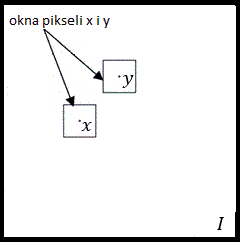
\includegraphics[scale=1]{rysunki/3_fig3.png}
	\caption{Kształt okien wykorzystywanych do obliczania wartości $w(x,y)$.}
	\label{3_fig3}
\end{figure}
Wartość $r$ to uprzednio definiowana stała skalująca wartości podobieństwa pomiędzy pikselami. Podobieństwo wyznaczane jest na podstawie utworzonych okien scentrowanych względem piksela $x$ oraz $y$ oznaczanych operatorem "$\cdot$" zgodnie z \autoref{3_fig3}. Normę macierzową występującą w powyższej zależności można wyznaczyć korzystając z normy Frobeniusa:
\begin{equation}
{\left|I\left(x+\ \cdot \right)-I\left(y+\ \cdot \right)\right|}^2=\ \sum^n_{i=1}{\sum^n_{j=1}{{\left(I_{x+\ \cdot }\left(i,j\right)-I_{y+\ \cdot }\left(i,j\right)\right)}^2}}
\label{FROBENIUS}
\end{equation}
gdzie wartość $n$ odpowiada wielkości badanego okna i stanowi uprzednio definiowany parametr. Zmienna $G_\sigma$ reprezentuje macierz o rozmiarze zgodnym z operatorem otoczenia danego piksela "$\cdot$". Wartości wewnątrz macierzy pozwalają stopniować wpływ każdego z rozpatrywanych pikseli na uzyskiwany wynik poprzez przyznawanie większego priorytetu pikselom centralnym, przy deprecjonowaniu tych bardziej oddalonych od centrum. Podobnie jak w przypadku nielokalnego gradientu funkcja wagi stanowi mapowanie $DxD\longrightarrow R$. Kolejnymi ważnymi nielokalnymi operatorami wykonanymi w punkcie $x$ są: 
\begin{itemize}
\item
iloczyn skalarny dwóch nielokalnych mapowań $\overrightarrow{p}:DxD\longrightarrow R$ (mapowaniem $\overrightarrow{p}$ może być wspomniana funkcja wagi, bądź nielokalny gradient):
\begin{equation}
\left({\overrightarrow{p}}_1\cdot {\overrightarrow{p}}_2\right)(x)\triangleq \int_D{p_1(x,y)\cdot p_2\left(x,y\right)dy}
\label{NLPRODUCT}
\end{equation}
\item
moduł mapowania $\overrightarrow{p}$:
\begin{equation}
\left|\overrightarrow{p}\right|\left(x\right)\triangleq \sqrt{\overrightarrow{p}\cdot \overrightarrow{p}}=\sqrt{\int_D{{\left(p\left(x,y\right)\right)}^2dy}} 
\label{NLMOD}
\end{equation}
\item
dywergencja mapowania $\overrightarrow{p}$:
\begin{equation}
({\mathrm{\nabla }}_{NL}\cdot \overrightarrow{p})(x)\ \triangleq \int_D{\left(p\left(x,y\right)-p\left(y,x\right)\right)\sqrt{w(x,y)}dy}
\label{NLDIV}
\end{equation}
\item
laplasjan mapowania
\begin{equation}
{\mathrm{\Delta }}_{NL}\overrightarrow{p}(x)\ \triangleq \frac{1}{2}{\mathrm{\nabla }}_{NL}\cdot \left({\mathrm{\nabla }}_{NL}I\left(x\right)\right)=\int_D{\left(I\left(y\right)-I\left(x\right)\right)w(x,y)dy}
\label{NLLAP}
\end{equation}
\end{itemize}
Warto zauważyć, iż w przypadku mapowań w postaci nielokalnego gradientu \eqref{NLGRAD} oraz wagi \eqref{NLWEIGHT} zachodzą odpowiednio zależności:
\begin{align}
\left(p\left(x,y\right)-p\left(y,x\right)\right) &= \left({\mathrm{\nabla }}_{NL}I\left(x,y\right)-{\mathrm{\nabla }}_{NL}I\left(y,x\right)\right)  \notag \\ 
&= \left({\mathrm{\nabla }}_{NL}I\left(x,y\right)+{\mathrm{\nabla }}_{NL}I\left(x,y\right)\right) \notag \\
&=2{\mathrm{\nabla }}_{NL}I\left(x,y\right)\
\label{NLPOM}
\end{align}
Stąd w szczególnym przypadku nielokalną dywergencję można przedstawić: 
\begin{equation}
({\mathrm{\nabla }}_{NL}\cdot \overrightarrow{p})(x)\ \triangleq \int_D{2\left(p\left(x,y\right)\right)\sqrt{w(x,y)}dy}
\label{NLDIVSMART}
\end{equation}
\begin{equation}
w(x,y) = w(y,x)
\label{SMARTWEIGHT}
\end{equation}
Nielokalna dywergencja stanowi mapowanie $DxD\longrightarrow D$.
W celu dyskretyzacji powyższych równań należy zgodnie z \cite{gilboa2008nonlocal} wprowadzić pojęcie okna poszukiwania ${\mathrm{N}}_i$, gdzie $i\in D,\ j\in {\mathrm{N}}_i$. Rozmiar okna stanowi uprzednio definiowany parametr. Dla wszystkich pikseli w oknie zachodzi zależność ${\mathrm{N}}_i\coloneqq \left\{j:w_{i,j}>0\right\}$. Wprowadzenie okna skutkuje ograniczeniem wcześniej wprowadzonego mapowania $DxD\longrightarrow R$ do $\mathrm{N}xD\longrightarrow R$.
\begin{figure}[!h]
	\centering
	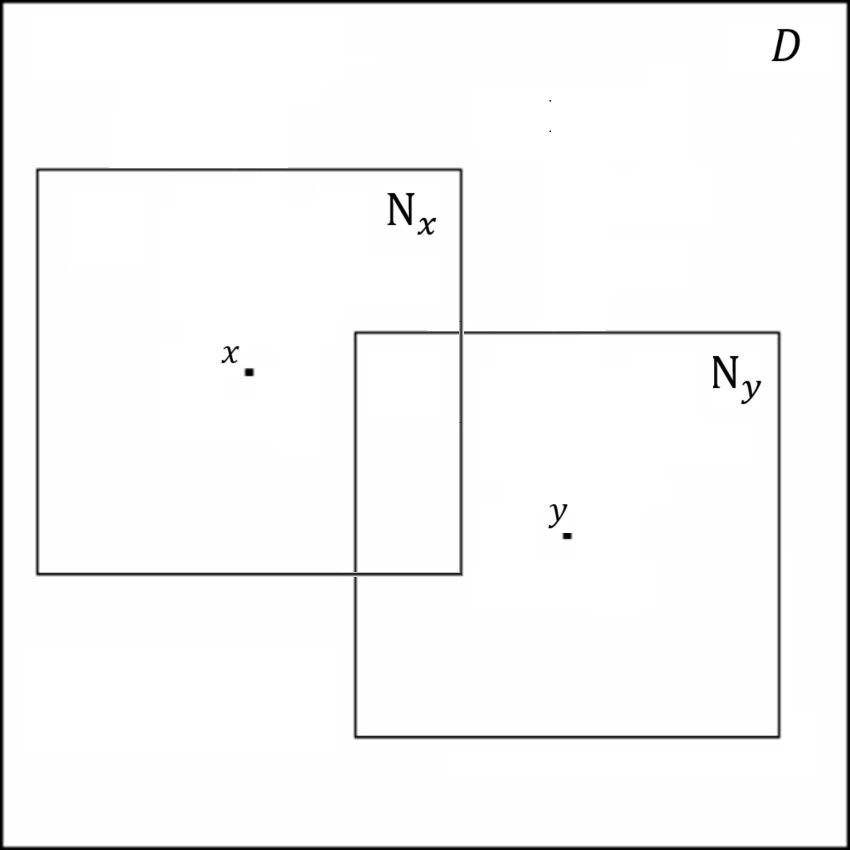
\includegraphics[scale=0.5]{rysunki/3_fig4.png}
	\caption{Przykładowe okna ${\boldsymbol{\mathrm{N}}}_{\boldsymbol{x}}\boldsymbol{,\ }{\boldsymbol{\mathrm{N}}}_{\boldsymbol{y}}$ utworzone dla pikseli $\boldsymbol{x},\boldsymbol{y}$.}
	\label{3_fig4}
\end{figure}
\par
Niech przypisy dolne wskazują na dyskretną lokalizację w przestrzeni obrazu $D$. Wtedy nielokalne operatory przedstawić można za pomocą zdyskretyzowanych równań:
\begin{equation}
{\mathrm{\nabla }}_{NLd}I_{i,j}\triangleq \left(I_j-I_i\right)\sqrt{w_{i,j}}
\label{DNLGRAD}
\end{equation}
\begin{equation}
w_{i,j}={\mathrm{exp} \left\{-\sum_{l\in G_{\sigma },j\in N_i,k\in N_j \\
}{{G_{\sigma }}_l\ast {\left|I_j-I_k\right|}^2}\right\}\ }
\label{DNLWEIGHT}
\end{equation}
\begin{equation}
{\left|\overrightarrow{p}\right|}_i\triangleq \sqrt{\sum_{j\in N_i \\ 
}{{\left(p_{i,j}\right)}^2}}
\label{DNLMAG}
\end{equation}
\begin{equation}
{\mathrm{\nabla }}_{NLd}\cdot \overrightarrow{p_i}\ \triangleq \sum_{ 
j\in N_i \\ 
}{\left(p_{i,j}-p_{j,i}\right)}\sqrt{w_{i,j}}
\label{DNLDIV}
\end{equation}
\begin{equation}
{\mathrm{\Delta }}_{NL}{\overrightarrow{p}}_i\ \triangleq \sum_{
j\in N_i \\ 
}{\left(I_j-I_i\right)}w_{i,j}
\label{DNLLAP}
\end{equation}
W szczególnym przypadku dla \eqref{NLDIVSMART} można zapisać:
\begin{equation}
{\mathrm{\nabla }}_{NLd}\cdot \overrightarrow{p_i}\ \triangleq \sum_{ 
j\in N_i \\ 
}{2p_{i,j}}\sqrt{w_{i,j}}
\label{DNLDIVSMART}
\end{equation}
Warto zauważyć, iż indeksy $i,j$ wskazują na konkretny piksel w obrazie. Lokalizacji w przestrzeni $2D$ dokonuje się przez znajomość par: $i=(x_i,y_i)$ oraz $j=(x_j,y_j)$, gdzie $x$ oś rzędnych, odpowiednio $y$ oś odciętych.
\par 
Nielokalny model wahania funkcji oznaczany $NL-TV$ definiowany dla obrazów w odcieniach szarości przyjmuje następująca postać:
\begin{equation}
{\mathop{\mathrm{min}}_{u} \left\{E\left(u\right)=\ \int_D{\left|{\mathrm{\nabla }}_{NL}u(x)\right|}dx+\frac{1}{2}\int_D{{\lambda }_d{\left(u-f\right)}^2}dx\ \right\}\ }
\label{NLTVGRAY}
\end{equation}
gdzie $f$ stanowi oryginalny obraz wejściowy $f\left(x\right):D\mathrm{\longrightarrow }\mathrm{R}$, natomiast $u\left(x\right):D\mathrm{\longrightarrow }\mathrm{R}$ obraz wynikowy, będący obrazem wmalowanym, bądź w przypadku pierwotnych założeń obrazem z usuniętym szumem. W przypadku wmalowywania zmienna ${\lambda }_d$ to funkcja definiowana na podstawie maski obrazu przyjmująca następujące wartości:
\begin{equation}
{\lambda }_d\left(x\right)=\left\{ \begin{array}{c}
0\ x\ \epsilon \ \mathrm{\Omega } \\ 
1\ x\ \epsilon \ D/\mathrm{\Omega } \end{array}
\right\}
\end{equation}
Tak zdefiniowany model można przekształcić wykorzystując operację rozbicia Bregman’a. Rozbicie stosuje się w celu poprawienia wydajności obliczeniowej w przypadku dyskretnej implementacji problemu minimalizacji energii. Wprowadzenie pomocniczej zmiennej $\overrightarrow{v}=v\left(x,y\right):\ \mathrm{\Omega }\mathrm{\ }x\ \mathrm{\Omega }\longrightarrow R$ i parametru Bregman’a $\overrightarrow{b}=\overrightarrow{b}\left(x,y\right):\ \mathrm{\Omega }\mathrm{\ }x\ \mathrm{\Omega }\longrightarrow R$ pozwala przekształcić problem minimalizacji powyższej energii do następującej postaci iteracyjnej:
\begin{align}
\begin{aligned}
\left(u^{k+1},{\overrightarrow{v}}^{k+1}\right) &= arg\ \mathop{\mathrm{min}}_{u,\overrightarrow{v}} E\left(u,\overrightarrow{v}\right)\\ 
&= \biggl\{arg\ \mathop{\mathrm{min}}_{u,\overrightarrow{v}}
\int_D{|\overrightarrow{v}|\left(x\right)}dx+\frac{1}{2}\int_D{{\lambda }_d{\left(u-f\right)}^2}dx \\
&+  \frac{\mathrm{\Theta }}{2}\int_D{{\left|\overrightarrow{v}-{\mathrm{\nabla }}_{NL}u-{\overrightarrow{b}}^{k+1}\right|}^2(x)}dx\ \biggr\}
\end{aligned}
\label{NLTVGRAYMINPROB}
\end{align}
\begin{align}
{\overrightarrow{b}}^{k+1}={\overrightarrow{b}}^k+{\mathrm{\nabla }}_{NL}u^k-{\overrightarrow{v}}^k, {\overrightarrow{b}}^0={\overrightarrow{v}}^0=0
\label{BREGMANVARIABLE}
\end{align}
gdzie $\Theta$ stanowi uprzednio definiowany parametr algorytmu. Stosując podstawowe równanie rachunku wariacyjnego postaci równania Eulera-Lagrange’a, metodę przedstawioną w \cite{tai2011fast} oraz schemat iteracyjny Gauss’a-Seidel’a powyższe równania można sprowadzić do problemu iteracyjnego rozwiązania poniższych zależności:
\begin{align}
{\lambda }_D\left(u-f\right)+\mathrm{\Theta }{\mathrm{\nabla }}_{NL}\cdot \left({\overrightarrow{v}}^k-{\mathrm{\nabla }}_{NL}u-{\overrightarrow{b}}^{k+1}\right)=0
\label{ELNLTV1}
\end{align}
\begin{align}
{\overrightarrow{v}}^{k+1}\mathrm{=}{\mathrm{max} \left(\left|{\mathrm{\nabla }}_{NL}u^{k+1}+{\overrightarrow{v}}^{k+1}\right|-\frac{1}{\mathrm{\Theta }},0\right)\cdot\frac{{\mathrm{\nabla }}_{NL}u^{k+1}+{\overrightarrow{b}}^{k+1}}{\left|{\mathrm{\nabla }}_{NL}u^{k+1}+{\overrightarrow{b}}^{k+1}\right|}\ }
\label{ELNLTV2}
\end{align}
Zależności można stosować dla obrazów w odcieniach szarości, bądź obrazów kolorowych traktując każdą z poszczególnych warstw osobnym algorytmem iteracyjnym. Zgodnie z \cite{duan2015fast} takie rozwiązanie prowadzi do niezachowania odpowiedniego kontrastu odrestaurowanej części obrazu i niezachowania krawędzi.
\par
W celu uzależnienia od siebie wszystkich warstw obrazu autorzy w \cite{duan2015fast} proponują zastosowanie funkcjonału MTV przedstawionego w \cite{yang2009fast}, funkcjonału $CTV$ przedstawionego w \cite{blomgren1998color}, bądź model Mumford-Shah’a dokładnie opisanego w \cite{jung2011nonlocal}. Ze względu na wydajniejszą implementację oraz najlepsze wyniki uzyskiwane w przypadku modelu $CTV$ został on wybrany do badań w niniejszej pracy. Wykorzystując wspomniany funkcjonał energia przyjmuje postać:
\begin{align}
{\mathop{\mathrm{min}}_{u} \left\{E\left(u\right)=\sqrt{\sum^m_{i=1}{{\left(\int_D{\left|{\mathrm{\nabla }}_{NL}u(x)\right|}dx\right)}^2}\ }\ +\frac{1}{2}\sum^m_{i=1}{\int_D{{\lambda }_d{\left(u_i-f_i\right)}^2}dx}\ \right\}\ }
\label{ENLCTV}
\end{align}
gdzie $m$ odpowiada ilości warstw tworzących kolorowy obraz. Zastosowanie równania rachunku wariacyjnego postaci Eulera-Lagrange’a w swoim rozwiązaniu prowadzi do konieczności obliczenia nielokalnej krzywizny krzywej, będącej w przypadku dyskretyzacji rozwiązania znacznie obciążającą obliczeniowo operacją. W tym celu, podobnie jak w przypadku poprzedniego modelu $NL-TV$ zastosowany zostanie heurystyczny algorytm rozbicia Bregman’a. Analogicznie wprowadzone zostają zmienne $\overrightarrow{v}=\left({\overrightarrow{v}}_1,{\overrightarrow{v}}_2,\ \dots ,\ \ {\overrightarrow{v}}_m\right)$ oraz $\overrightarrow{b}=\left({\overrightarrow{b}}_1,{\overrightarrow{b}}_2,\ \dots ,\ \ {\overrightarrow{b}}_m\right)$. Wtedy przytoczona energia przyjmuje iteracyjną postać: 
\begin{align}
\begin{aligned}
\mathop{\mathrm{min}}_{u}E\left(u\right) &= \mathop{\mathrm{min}}_{u}\Biggl\{\sqrt{\sum^m_{i=1}{{\left(\int_D{\left|\overrightarrow{v_i}\right|(x)}dx\right)}^2}\ }\\ 
&+\frac{1}{2}\sum^m_{i=1}{\int_D{{\lambda }_d{\left(u_i-f_i\right)}^2}dx} 
+\frac{\theta }{2}\sum^m_{i=1}{\int_D{{\left|\overrightarrow{v_i}-{\mathrm{\nabla }}_{NL}u_i-\ {\overrightarrow{b_i}}^{k+1}\right|}^2\left(x\right)}dx}\Biggr\}
\end{aligned}
\label{ENLCTV1}
\end{align}
\begin{align}
{\overrightarrow{b_i}}^{k+1}={\overrightarrow{b_i}}^k+{\mathrm{\nabla }}_{NL}u^k_i-{\overrightarrow{v_i}}^k,\ {{\overrightarrow{b}}_i}^0={\overrightarrow{v_i}}^0=0
\label{ENLCTV2}
\end{align}
Przyjmując naprzemienną strategię minimalizacji energii można uzyskać równania Eulera-Lagrange’a wyznaczone oddzielnie względem zmiennych $u$ oraz $v$:
\begin{align}
{\lambda }_D\left(u_i-f_i\right)+\mathrm{\Theta }{\mathrm{\nabla }}_{NL}\cdot \left({\overrightarrow{v_i}}^k-{\mathrm{\nabla }}_{NL}u_i-{{\overrightarrow{b}}_i}^{k+1}\right)=0
\label{ELNLCTV1}
\end{align}
\begin{align}
\mathrm{\Theta }\left(\overrightarrow{v_i}\mathrm{-}{\mathrm{\nabla }}_{NL}u^{k+1}_i\mathrm{-}{{\overrightarrow{b}}_i}^{k+1}\right)\mathrm{+}\frac{\int_D{\left|\overrightarrow{v_i}\right|(x)}dx}{\sqrt{\sum^m_{i=1}{{\left(\int_D{\left|\overrightarrow{v_i}\right|(x)}dx\right)}^2}\ }}\frac{\overrightarrow{v_i}}{\left|\overrightarrow{v_i}\right|(x)}\mathrm{=0}
\label{ELNLCTV2}
\end{align}
W celu przedstawienia dyskretnej formy równań \eqref{ELNLCTV1} i  \eqref{ELNLCTV2} i \eqref{ELNLCTV2} wygodnym będzie zapis dla konkretnego piksela $l\in D$ w obrazie. W przypadku \eqref{ELNLCTV1}: 
\begin{align}
{\left({\lambda }_D\right)}_l\ \ \left[{\left(u_i\right)}_l-{\left(f_i\right)}_l\right]+\mathrm{\Theta }{\mathrm{\nabla }}_{NL}\cdot \left[{\left({\overrightarrow{v_i}}^k\right)}_l-{\left({\mathrm{\nabla }}_{NL}u_i\right)}_l-{\left({{\overrightarrow{b}}_i}^{k+1}\right)}_l\right]=0
\label{DELNLCTV1}
\end{align}
Korzystając z dyskretnych form \eqref{NLGRAD}, \eqref{NLWEIGHT}, \eqref{NLPRODUCT} i \eqref{NLDIV} równanie \eqref{ELNLCTV1} można przedstawić w postaci:
\begin{align}
\begin{aligned}
{{\left(u_i\right)}_l}^{k+1} &= \frac{1}{{\left({\lambda }_D\right)}_l+2\mathrm{\Theta} \sum\limits_{j\in N_i} {\left(w_i\right)}_{l,j}\ } \Biggl[2\mathrm{\Theta }\sum_{j\in N_i} {{{\left(u^k_i\right)}_j\left(w_i\right)}_{l,j}\ }\\
&+ {\left({\lambda }_D\right)}_l{\left(f_i\right)}_l \\
&-\mathrm{\Theta} \Biggl( \sum_{j\in N_i} \left( \left({ v^k_i}\right)_{l,j} - (\left({ v^k_i}\right)_{l,j} - (\left({ v^k_i}\right)_{l,j} + (\left({ v^k_i}\right)_{l,j}\right) \sqrt{{\left(w_i\right)}_{l,j}} \Biggr]
\end{aligned}
\end{align}
W przypadku równania \eqref{ELNLCTV1} Eulera-Lagrange’a należy przekształcić je względem zmiennej $\overrightarrow{v}$:
\begin{align}
\begin{aligned}
{\overrightarrow{v_i}}^{k+1} &= \mathrm{max} \left(\left|{\mathrm{\nabla }}_{NL}u^{k+1}_i+{\overrightarrow{b_i}}^{k+1}\right|-\frac{\int_D{\left|\overrightarrow{v_i}\right|(x)}dx}{\mathrm{\Theta }\sqrt{\sum^m_{i=1}{{\left(\int_D{\left|{\overrightarrow{v_i}}^k\right|(x)}dx\right)}^2}\ }},0\right) \\ 
&\cdot \frac{{\mathrm{\nabla }}_{NL}u^{k+1}_i+{{\overrightarrow{b}}_i}^{k+1}}{\left|{\mathrm{\nabla }}_{NL}u^{k+1}_i+{\overrightarrow{b_i}}^{k+1}\right|}\ 
\label{DELNLCTV2}
\end{aligned}
\end{align}
Podobnie, korzystając z dyskretnych form \eqref{NLGRAD}, \eqref{NLWEIGHT}, \eqref{FROBENIUS}, \eqref{NLPRODUCT} i \eqref{NLDIV} równanie \eqref{DELNLCTV2} można przedstawić w postaci:
\begin{align}
{\left({\overrightarrow{v_i}}^{k+1}\right)}_l\cong {\mathrm{max} \left({\left|A^{k+1}_i\right|}_l-\frac{B^k_i}{\mathrm{\Theta }\sqrt{\sum^m_{i=1}{{\left(B^k_i\right)}^2}\ }},0\right)\frac{{\left(A^{k+1}_i\right)}_l}{{\left|A^{k+1}_i\right|}_l}\ }
\label{VNLCTVITER}
\end{align}
gdzie:
\begin{align}
{\left(A^{k+1}_i\right)}_l=\left({\left(u^{k+1}_i\right)}_j-{\left(u^{k+1}_i\right)}_l\right)\sqrt{{\left(w_i\right)}_{l,j}}+{\left(b^{k+1}_i\right)}_{l,j}
\end{align} 
\begin{align}
{\left|A^{k+1}_i\right|}_l=\sqrt{\sum_j{{\left(\left({\left(u^{k+1}_i\right)}_j-{\left(u^{k+1}_i\right)}_l\right)\sqrt{{\left(w_i\right)}_{l,j}}+{\left(b^{k+1}_i\right)}_{l,j}\right)}^2}\ }
\end{align}
\begin{align}
B^k_i=\sum_l{\sqrt{\sum_j{{{\left(v^k_i\right)}^2}_{l,j}}}}
\end{align}
Warto przypomnieć, iż w przytoczonych wzorach $j$ odpowiada pikselom znajdującym się oknie poszukiwania ${\mathrm{N}}_l$ scentrowanym względem piksela $l$, a $i$ odpowiada $i$-tej warstwie spośród warstw tworzących obraz kolorowy. Autorzy w \cite{jung2011nonlocal} proponują zmodyfikowany sposób wyznaczania wagi uwzględniający kształt maski w obrazie:
\begin{align}
w\left(x,y\right)\triangleq {\mathrm{exp} \left\{-\frac{G_{\sigma }*{\chi }_R\left(x+\ \cdot \right){\left|I\left(x+\ \cdot \right)-I\left(y+\ \cdot \right)\right|}^2}{r^2}\right\}\ }
\label{NLWEIGHTMASK}
\end{align}
gdzie:
\begin{equation}
{\chi }_d\left(x\right)=\left\{ \begin{array}{c}
0\ x\ \epsilon \ \mathrm{\Omega } \\ 
1\ x\ \epsilon \ D/\mathrm{\Omega } \end{array}
\right\}
\end{equation}
Podsumowując algorytm wmalowywania w oparciu o model $NL-CTV$ z algorytmem rozbicia Bregman’a można przedstawić w następujących krokach:
\begin{enumerate}
\item  
Inicjalizacja zmiennych $k=0,\ \overrightarrow{b^0_i}=0,\ \overrightarrow{v^0_i}=0,\ u^0_i=f^0_i$ 
\item  
Wyznaczenie wagi $w^2_i$ zgodnie z \eqref{NLWEIGHTMASK} dla całego obszaru obrazu $D$
\item  
Powtarzanie do spełnienia kryterium końcowego:
\begin{itemize}
%\addtolength{\itemindent}{1cm}
\item
\noindent Wyznaczenie ${\overrightarrow{b}}^{k+1}={\overrightarrow{b}}^k+{\mathrm{\nabla }}_{NL}u^k-{\overrightarrow{v}}^k$
\item
\noindent Wyznaczenie $u^{k+1}$ na podstawie \eqref{DELNLCTV1} dla każdego piksela $l$
\item
\noindent Wyznaczenie $v^{k+1}$ na podstawie \eqref{VNLCTVITER} dla każdego piksela $l$
\end{itemize}
\item  
Aktualizacja wagi $w^2_i$ w obszarze $\mathrm{\Omega }$
\end{enumerate}
Kryterium definiującym zakończenie algorytmu może być uzyskanie granicznej wartości różnicy energii $\epsilon$ uprzednio definiowanej pomiędzy wykonywanymi iteracjami:
\begin{equation}
\left|E^{k+1}-E^k\right|\le \varepsilon
\end{equation}
\chapter{Uzupełnianie kawałkami obrazu}
Kolejną grupą algorytmów rozważanych w niniejszej pracy jest grupa opierająca się na wypełnianiu brakujących obszarów w obrazie skrawkami pochodzącymi z ich otoczenia. W odróżnieniu od metod bazujących na równaniach różniczkowych metoda uzupełniania braków nie bazuje na metodzie dyfuzji. Pierwszy raz zaproponowana została w \cite{efros1999texture}, a jej podstawowy krok opiera się na schemacie przedstawionym na poniższym rysunku.
\begin{figure}[!h]
	\centering
	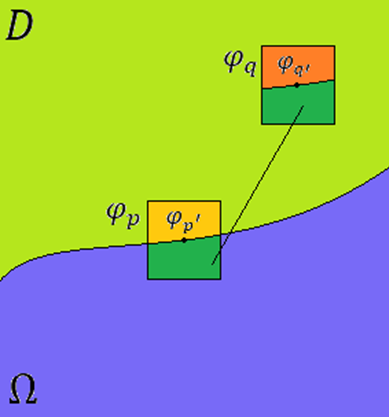
\includegraphics[scale=0.5]{rysunki/4_fig1}
	\caption{Schemat wmalowywania obrazu.}
	\label{4_fig1}
\end{figure}
Zgodnie z \autoref{4_fig1} niech zbiór $D$ oznaczony kolorem jasnozielonym określa znane punkty obrazu, natomiast $\omega $ oznaczony kolorem fioletowym określa obszar do odrestaurowania. Niech obraz wejściowy stanowi funkcję $\mathrm{\Omega }$. Niech ${\varphi}_p$ stanowi podzbiór punktów tworzących skrawek o uprzednio zdefiniowanej wielkości, scentrowany względem piksela $p$ znajdującego się na granicy maski $\partial \mathrm{\Omega }$. Niech ${\varphi}_q$ stanowi podzbiór punktów tworzących skrawek o rozmiarze równym rozmiarowi ${\varphi}_p$, scentrowany względem piksela $q$ dla którego żaden z punktów wyznaczonego skrawka nie znajduje się w obszarze maski. Niech ${\varphi}_{p'}$ oznaczone kolorem żółtym stanowi podzbiór punktów znajdujących się w ${\varphi}_p$, które nie znajdują się w obrębie maski. Wtedy ${\varphi}_{q'}$ oznaczone kolorem pomarańczowym stanowi grupę pikseli zlokalizowanych odpowiednio według pikseli z podzbioru ${\varphi}_{p'}$. Zgodnie z nomenklaturą matematyczną:
\begin{align}
p\ \epsilon \ \partial \mathrm{\Omega }
\end{align}
\begin{align}
q\ \epsilon \mathrm{\ }\phi 
\end{align}
\begin{align}
\phi \ \subset \ D
\end{align}
\begin{align}
{\varphi }_p=\mathrm{(p+\ }\mathrm{\cdot }\mathrm{)}
\end{align}
\begin{align}
{\varphi }_q=(q+\ \cdot )\ 
\end{align}
\begin{align}
{\varphi }_{p'}=\ {\varphi }_p\cap (D\cup W) 
\end{align}
\begin{align}
{\varphi }_{q'}\ \subset \ {\varphi }_q
\end{align}
gdzie $W$ przedstawia zbiór wmalowanych pikseli uprzednio znajdujących się w rejonie maski.
\par
Podstawową operacją wmalowywania metodą propagacji tekstury obrazu jest znalezienie najpodobniejszej pary $\left\langle {\ \varphi }_{p'},\ {\varphi }_{q''}\right\rangle $ oraz zgodnie z powyższym rysunkiem przepisanie wartości odpowiednich pikseli z wyznaczonego zbioru $({\varphi }_{(q^{''})}/{\varphi }_{(q^{''})'})$ do odpowiadających im pikseli w zbiorze $({\varphi }_p/{\varphi }_{p'})$ oznaczonych kolorem ciemnozielonym. Zapisując matematycznie:
\begin{align}
{\varphi }_{q^{''}}={\mathrm{arg}\ \mathop{\mathrm{min}}_{q\ \epsilon \mathrm{\ }\phi } d(\ }{\varphi }_{p'},{\varphi }_{q'})
\label{FROBDIST}
\end{align}
Dystans pomiędzy dwoma skrawkami $d({\varphi }_{p'},{\varphi }_{q'})$ definiowany jest jako suma kwadratów różnic wszystkich odpowiadających sobie pikseli ${\varphi }_{p'}$ oraz ${\varphi }_{q'}$.
\begin{align}
d(\varphi_{p'},\varphi_{q'})= \sum_{p\in \varphi_{p'}} \left( \varphi_{p^{'}}(p) - \varphi _{q^{'}} \left(p^{'}\right) \right)^2
\label{FROBENIUS} 
\end{align}


gdzie $\varphi \left(p\right)$ wartość jasności piksela $p$ z badanego okna. W celu odrestaurowania obrazu powyższy schemat powtarzany jest aż do momentu wypełnienia całego obszaru $\mathrm{\Omega }$.
Metoda wmalowywania pierwszy raz przedstawiona w  \cite{efros1999texture} nie zakłada żadnego priorytetu ani kolejności wypełniania braków ustalanej na podstawie otoczenia maski. Przeprowadzana synteza obrazu pomimo wyznaczenia dla danego piksela trafnego dopasowania może prowadzić do akumulowanej przez algorytm niespójności obrazu.
\begin{figure}[!h]
	\centering
	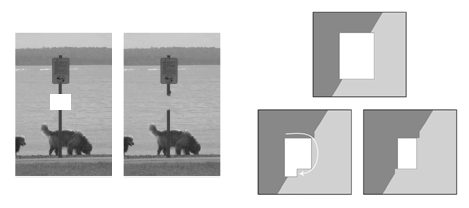
\includegraphics[scale=1]{rysunki/4_fig2}
	\caption{Wpływ prostego schematu wypełniania braków na wynikową teksturę obrazu. Źródło \cite{criminisi2004region}.}
	\label{4_fig2} 
\end{figure}
\par
W 2004 roku Criminisi w \cite{criminisi2004region} korzysta z koncepcji próbkowania kawałków obrazu proponując nowe podejście do wyznaczania kolejności ich wmalowywania.  Kolejność wypełniania wyznaczana jest na podstawie izolinii poziomu jasności obrazu. W każdej iteracji algorytmu dla pikseli sąsiadujących z maską wyznaczane są wartości priorytetu. Następnie wypełnienie odbywa się dla piksela o największym priorytecie. Dzięki nowemu podejściu izolinie będące granicami struktur obrazu są kontynuowane w miejsca odrestaurowywane.
\par
Algorytm przedstawiony w \cite{criminisi2004region} opiera się na powtarzaniu 3 głównych kroków w każdej iteracji wykonywanej do momentu wypełnienia wszystkich pikseli ze zbioru $\mathrm{\Omega }$. Każda kolejna iteracja prowadzi do przesunięcia granicy maski w jej głąb. W trakcie próbkowania kawałków obrazu zbiór $\phi $ będący źródłem próbkowania nie zmienia się. Pierwsze dwa kroki w pojedynczej iteracji służą wyznaczeniu priorytetu $P\left(p\right)$ dla każdego piksela obrazu znajdującego się na granicy maski $\partial \mathrm{\Omega }$, natomiast trzeci znalezieniu najlepszego dopasowania ${\varphi }_{q^{''}}$. Priorytet $P\left(p\right)$ każdego piksela $p$ znajdującego się na granicy maski wyznaczany jest z zależności:
\begin{align}
P\left(p\right)=Ct(p)\cdot Dt(p)
\label{PRIORITY}
\end{align}
Pierwszy krok w każdej wykonywanej iteracji związany jest z obliczenie wartości funkcji $Ct(p)$ definiowanej:
\begin{align}
Ct\left(p\right)=\ \frac{\sum_{q\in {\varphi }_{p'}}{C(q)}}{\left|{\varphi }_p\right|}
\end{align}
gdzie $C(q)$ - funkcja przypisująca wszystkim pikselom z obrazu poziom wiarygodności odwzorowania oryginalnego obrazu, $\left|{\varphi }_p\right|$ - liczba pikseli w analizowanym kawałku - rozmiar rozważanego okna. 
\par
Podczas inicjalizacji funkcja $C(q)$ dla każdego piksela stanowiącego oryginalny obraz przyjmuje wartość $1$, natomiast dla punktów maski przyjmuje 0. Matematycznie ${\forall }_{q\in D}\ C\left(q\right)=1$  i analogicznie ${\forall }_{q\in \mathrm{\Omega }}\ C\left(q\right)=0$. Wraz z wyznaczaniem kolejnych wartości pikseli z rejonu maski funkcja $C\left(q\right)$ jest aktualizowana, a zerowe wartości są nadpisywane. Funkcja $Ct\left(p\right)$ jest sumą wartości $C\left(p\right)\ $wszystkich pikseli z analizowanego skrawka scentrowanego względem piksela p, które znajdują się w przestrzeni wyznaczonego już obrazu podzielonej przez ilość pikseli w danym skrawku. Funkcję interpretuje się jako czynnik wymuszający koncentryczne, czyli postępujące wypełnianie wzdłuż granicy maski nieznanych punktów zgodnie z pierwotnym założeniem w \cite{efros1999texture}. Wynika to z pierwszeństwa jakie wprowadza funkcja $C\left(p\right)$ przypisując w każdej iteracji coraz niższe wartości kolejnym wypełnianym pikselom. W ten sposób pierwszeństwo wypełniania uzyskują wycinki obrazu zawierające większą liczbę pikseli wypełnionych w poprzednich iteracjach, bądź zawierających oryginalne części obrazu. Mniejsza wartość $C\left(p\right)$ w każdym kroku interpretuje się jako mniejszą pewność co do przepisanych wartości koloru w obrazie. Drugi krok w każdej wykonywanej iteracji związany jest z obliczenie wartości funkcji $D(p)$ definiowanej jako:
\begin{align}
D(p)=\ \frac{\left|{\mathrm{\nabla }}^{\bot }I_P\cdot n_p\right|}{\alpha }
\label{DataTerm}
\end{align}
gdzie człon ${\mathrm{\nabla }}^{\bot }I_P$ podobnie jak w przypadku równania Naviera-Stokes'a odpowiada kierunkowi rozchodzenia się izolinii obrazu, natomiast  $n_p$ to wektor normalny (prostopadły) do granicy maski $\partial \mathrm{\Omega }$ w punkcie piksela $p$.  
\begin{figure}[!h]
	\centering
	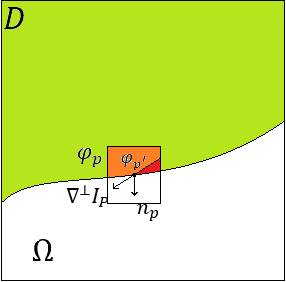
\includegraphics[scale=1]{rysunki/4_fig3}
	\caption{Oznaczenie wektorów wykorzystywanych do liczenia wartości $\boldsymbol{D}\left(\boldsymbol{p}\right)$.}
	\label{4_fig3} 
\end{figure}
Zgodnie z \autoref{4_fig3} funkcja $D\left(p\right)$ w sposób liczbowy określa z jaką siłą izolinia obrazu uderza granicę maski. Ta zalebna jest od gradientu jasności obrazu ${\mathrm{\nabla }}^{\bot }I_P$ oraz orientacji względem gradientu wektora normalnego do granicy maski. Funkcja przyjmuje największą wartość w momencie, w którym wektor normalny oraz wektor izolinii są do siebie równoległe (zgodnie z iloczynem skalarnym wektorów ${\mathrm{cos} 0^0\ }=1)$, a człon ${\mathrm{\nabla }}^{\bot }I_P$ ma największą wartość. W przeciwieństwie do definicji terminu $Ct(p)$ funkcję $D(p)$ można zinterpretować jako człon odpowiedzialny za przyznanie wyższego priorytetu pikselowi, stanowiącemu część struktury, która według psychologii widzenia powinna być kontynuowana w głąb odrestaurowywanego obszaru. Funkcja $D(p)$ wpływa ma zmniejszenie pojawiającego się w metodzie zjawiska wprowadzania niespójności obrazu. Niech funkcja $M$ w punktach oryginalnego obrazu $D$ przyjmuje wartość 0 oraz w punktach maski w punktach $\mathrm{\Omega }$ wartość 1, $I:D\to \{0,1\}$.  Wtedy korzystając z zależności \eqref{dfdx} i \eqref{dfdy} wektor normalny do granicy maski można wyznaczyć z zależności:
\begin{align}
n_p=\ \ \left[-n_x\frac{1}{L}\ ,\ -n_y\frac{1}{L}\right]\ =\ \left[-\frac{M_{i+1,j}+M_{i-1,j}}{2h}\cdot \frac{1}{L}\ ,\ -\frac{M_{i,j+1}+M_{i,j-1}}{2h}\cdot \frac{1}{L}\right]
\label{KIERUNEK}
\end{align}
\begin{align}
L=\ \sqrt{n^2_x+\ n^2_y}
\label{POMKIERUNEK}
\end{align}
Postać dyskretna równania \eqref{DataTerm} zgodnie z \eqref{u}, \eqref{v}, \eqref{KIERUNEK} i \eqref{POMKIERUNEK} przyjmuje postać:
\begin{align}
D(p)=\ \left|u{\cdot n}_x\frac{1}{L}-v\cdot n_y\frac{1}{L}\right|
\end{align}
Znając wartości $Ct\left(p\right)$ oraz $D(p)$ dla każdego piksela z granicy maski można wyznaczyć wartość priorytetów $P(p)$. Na ich podstawie wybierane jest okno ${\varphi }_p$, a następnie najlepsze odwzorowanie ${\varphi }_{q^{''}}$. Ze względu na nieregularny kształt większości masek wyznaczenie jej granicy $\partial \mathrm{\Omega }$ można wykonać poprzez operację erozji i dylacji na funkcji $M$. Innym sposobem może być zastosowanie dyskretnego splotu maski $M$ z macierzą $mL\ $reprezentującą Laplasjan dla siatki 8-spójnej: 
\begin{equation}
mL=\left| \begin{array}{ccc}
1 & 1 & 1 \\ 
1 & -8 & 1 \\ 
1 & 1 & 1 \end{array}
\right|	
\label{LAPLASJAN}
\end{equation}
Podsumowując operację wmalowywania obrazu można przedstawić następującym algorytmem. Powtarzać aż do wypełnienia wszystkich pikseli z $\mathrm{\Omega }$:
\begin{enumerate}
\item
Na podstawie \eqref{LAPLASJAN} wyznaczyć granicę maski $\mathrm{\partial }\mathrm{\Omega }$
\item
Na podstawie \eqref{PRIORITY} wyznaczyć priorytety wszystkich pikseli z granicy maski $\mathrm{\partial }\mathrm{\Omega }$
\item
Na podstawie \eqref{FROBENIUS} wyznaczyć najlepsze dopasowanie dla okna utworzonego na podstawie punktu 2 
\item
Zgodnie z \autoref{4_fig1} przepisać wartości z okna najlepszego dopasowania w odrestaurowywany obszar, jednocześnie aktualizując wartości $C(p)$ zgodnie z zależnością:
\begin{align}
C\left(p\right)=C\left(\dot{p}\right)
\end{align} 
gdzie $p\in \ {\varphi }_p\cap \ \mathrm{\Omega }$, a $C\left(\dot{p}\right)$ to deprecjonowana wartość w każdej kolejnej iteracji.
\end{enumerate}
Poprawa algorytmu przedstawiona w \cite{criminisi2004region} prowadzi do polepszenia otrzymywanych wyników, lecz nie w optymalnym stopniu. W celu dalszej minimalizacji uzyskiwanych niespójności w obrazie i optymalizacji pod kątem szybkości działania algorytmów zostały wprowadzone kolejne modyfikacje: \cite{StructurePropagationManual} \cite{malluvalasaimplementation} \cite{SalientStrucTexProp}. 
Jednym z istotnych ulepszeń algorytmu wmalowywania w oparciu o kopiowanie kawałków jest wprowadzenie zależności kolejności ich wstawiania w oparciu o główne struktury w obrazie. W niniejszej pracy zaimplementowano i sprawdzono odrestaurowywanie obrazu na podstawie zadawanych ręcznie przez użytkownika głównych linii zgodnie z \cite{StructurePropagationManual}. Różnica pomiędzy zwykłym algorytmem przedstawionym w \cite{criminisi2004region}, a nowym rozwiązaniem polega na wstępnej definicji przez użytkownika grupy punktów znajdujących się w masce. Najczęściej są to krzywe, które zgodnie z psychologią widzenia powinny być kontynuowane w głąb maski tworząc odpowiednie połączenia między sobą. Krzywe charakteryzują się ograniczoną grupą pikseli mogących stanowić źródło uzupełniania maski. Ograniczając pole $\phi $ dla każdej kontynuowanej znacznie przyspiesza się krok iteracji związany z odnalezieniem najlepszej pary dopasowania ${\varphi }_{p'}$ oraz ${\varphi }_{q'}$. Schemat wmalowywania w oparciu o powyższy schemat przedstawia poniższy rysunek.
\begin{figure}[!h]
	\centering
	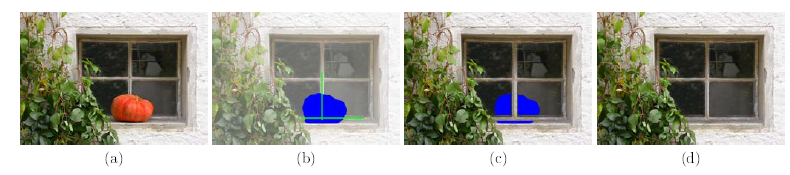
\includegraphics[scale=0.8]{rysunki/4_fig4}
	\caption{Koncepcja wmalowywania w oparciu o główne struktury obrazu. Źródło \cite{StructurePropagationManual}}
	\label{4_fig4} 
\end{figure}
W celu zaprojektowania w pełni automatycznego programu do procesu wmalowywania opierającego się na algorytmie wprowadzonym przez Criminisi zaproponowano dodatkową analizę obrazu ograniczającą interakcję użytkownika wyłącznie do wprowadzenia maski. Autorzy w \cite{SalientStrucTexProp} proponują wykonać 2 dodatkowe kroki:
\begin{enumerate}
\item
Wyznaczenie głównych struktur obrazu.
\item
Rozwiązanie poniższych zależności:
\begin{align}
D(i,j)\triangleq IP\cdot \left[\alpha \cdot D_1\left(f^i_C,f^j_C\right)\ +\ \beta {\cdot D}_2\left(f^i_T,f^j_T\right)+\gamma {\cdot D}_3\left(f^i_{Cur},f^j_{Cur}\right)\right]
\label{SalientDistance}
\end{align}
\begin{align}
Paired\left(i,j\right)={\mathrm{arg}\ \mathop{\mathrm{min}}_{i,j\ \epsilon \mathrm{\ }\{1,..,N\}} D(i,j)\ }
\label{SalientPair}
\end{align}
\end{enumerate}
Analiza powyższych równań wykonana zostanie w szczegółowy sposób dla każdego z członów $\alpha \cdot D_1\left(f^i_C,f^j_C\right)\ $,$\ \beta {\cdot D}_2\left(f^i_T,f^j_T\right)$, oraz $\gamma {\cdot D}_3\left(f^i_{Cur},f^j_{Cur}\right)$. Uprzednim krokiem do powyższych równań według \cite{SalientStrucTexProp} jest wyznaczenie głównych struktur na podstawie obrazu wejściowego poddanemu wstępnemu rozmyciu funkcją Gaussa:
\begin{align}
G\left(x,y\right)=\frac{1}{\sqrt{2\pi }\sigma }e^{\frac{x^2+y^2}{2{\sigma }^2}}
\label{rozmycieGaussa}
\end{align}
Operacji rozmycia dokonuje się poprzez operację splotu obrazu z odpowiednio wygenerowaną macierzą wyznaczoną na podstawie powyższego równania. Operacja rozmycia pozwala pozbyć się mniej znaczących krawędzi z obrazu zostawiając tylko najistotniejsze cechy, które powinny być kontynuowane w niewyznaczony obszar. Po operacji rozmycia autorzy w \cite{SalientStrucTexProp} proponują wykrycie głównych struktur na podstawie transformacji falkowej oraz odpowiednio wyznaczonych lokalnych maksimów dla funkcji powstałych na podstawie wspomnianej transformacji. Na podstawie przeprowadzonej operacji uzyskuje się wszystkie główne struktury obrazu. Zbiorem krawędzi poddanych do analizy są ostatecznie struktury, dla których dochodzi do przecięcia ze zdefiniowaną maską $\mathrm{\Omega }$ zgodnie z poniższym rysunkiem (jako maska traktowany jest samochód).
\begin{figure}[!h]
	\centering
	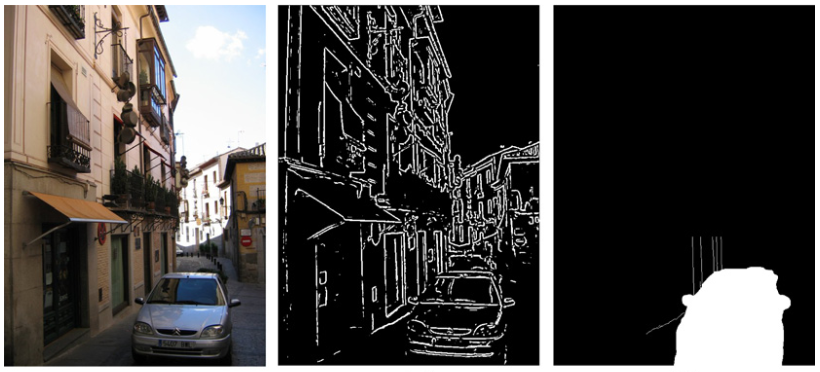
\includegraphics[scale=0.8]{rysunki/4_fig5}
	\caption{Koncepcja wmalowywania w oparciu o główne struktury obrazu. źródło \cite{StructurePropagationManual}.}
	\label{4_fig5} 
\end{figure}
Dla każdej linii stykającej się z obszarem $\mathrm{\Omega }$ wyznaczony zostaje punkt środkowy. Względem środka tego punktu tworzone jest okno  $f^i$ o uprzednio zdefiniowanym obszarze. Pierwszym członem w równaniu [4.19][4.19] wyznaczonym na podstawie utworzonego okna $f^i$ jest $D_1\left(f^i_C,f^j_C\right)$. Symbole $f^i_C$ oraz $f^j_C$ stanowią posegmentowane fragmenty obrazu względem uprzednio zdefiniowanej liczby głównych, dominujących kolorów w obrazie $M$. Dla każdego wycinka $f^i_C$ można zdefiniować zbiór punktów $(c_k,p_k)$, gdzie $c_k$ odpowiada danemu kolorowi, $p_k$ jego procentowemu udziałowi we fragmencie $f^i$, gdzie $k=1,\dots ,M$. Dysponując zbiorami punktów dla okien $f^i_C$,$\ f^j_C$ można liczbowo przedstawić ich poziom podobieństwa obliczając: 
\begin{align}
D_1\left(f^i_C,f^j_C\right)=IOCCD({\left(c_k,p_k\right)}_i,{\left(c_k,p_k\right)}_j
\end{align}
Dokładna analiza oraz sposób wyznaczania podobieństwa okien $f^i$ przedstawiony jest w \cite{chen2005adaptive}. 
 Drugim członem w równaniu [4.19][4.19] jest $D_2\left(f^i_T,f^j_T\right)$ określający stopień podobieństwa tekstur znajdujących się w utworzonych oknach $f$. Dla każdego obszaru $f^i$ z wyznaczonego zbioru okien wyznaczana jest macierz $MR8(f^i)$. Macierz uzyskiwana jest ma podstawie odpowiedzi fragmentu obrazu na grupę 38 filtrów przedstawionych na poniższym rysunku.
\begin{figure}[!h]
	\centering
	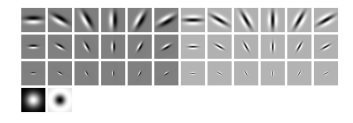
\includegraphics[scale=1]{rysunki/4_fig6}
	\caption{Bank 38 filtrów grupy MR8. źródło \cite{varma2009statistical}.}
\label{4_fig6}
\end{figure}
Przez odpowiedź obrazu na filtr należy rozumieć operację splotu z macierzą odpowiadającą definicji konkretnego filtru. W grupie filtrów $MR8$ branych pod uwagę znajduje się filtr Gaussowski, oraz filtr $LOG$ będący laplasjanem funkcji gaussowskiej. Na pozostałe 36 filtrów składają się dwie grupy filtrów utworzonych na podstawie filtru krawędziowego oraz filtru prętowego. Każdy z nich przedstawiony jest w sześciu orientacjach oraz 3 skalach zgodnie z rysunkiem \autoref{4_fig6}. Jako maksymalną odpowiedź na bazę trzydziestu ośmiu filtrów rozumie się zależność:
\begin{align}
I_{fmax}(p)=\mathrm{max}\mathrm{}(I_{f1}(p),I_{f2}(p),\dots ,I_{f38}(p))
\end{align}
gdzie $p$ - piksel obrazu poddanego filtracji, $p\in I$, $I_{fi}$ - odpowiedź obrazu $I$ na $i$-ty filtr z bazy filtrów. Podobieństwo wyznaczonych okien odpowiadających głównym strukturom w obrazie można wyrazić zależnością:
\begin{align}
D_2{\left(f^i_T,f^j_T\right)}_i=\frac{{\left|MR8\left(f^i\right)-MR8\left(f^j\right)\right|}_F}{250}=\frac{{\left|f^i_T-f^j_T\right|}_F}{250}
\end{align}
W powyższej zależności norma oznaczona literą $F$ odpowiada normie Frobenius'a liczonej następująco:
\begin{align}
\left|I\right|=\ \sqrt{\sum_{p\in I}{{\left|I\left(p\right)\right|}^2}}=\sqrt{{\sum^m_{i=1}{\sum^n_{j=1}{\left(f^i_T(i,j)-f^j_T(i,j)\right)}}}^2}
\end{align}
Dokładny algorytm klasyfikacji tekstur przedstawiony został przez Manika Varma'e i Adrew Zisserman'a w \cite{varma2009statistical}. Ostatnim członem w równaniu \eqref{SalientDistance} jest człon $D_3\left(f^i_{cur},f^j_{cur}\right)$ odpowiadający liczbowej reprezentacji podobieństwa krzywizn ze zbioru głównych struktur. Autorzy w \cite{SalientStrucTexProp} nie podają sposobu wyznaczenia normy:
\begin{align}
D_3\left(f^i_{cur},f^j_{cur}\right)=\ \left|curvature_i-curvature_j\right|
\end{align}
Proponują natomiast każdą z wyznaczonych głównych struktur przedstawić w postaci równania wielomianu drugiego stopnia. Aproksymacji współczynników wielomianu można dokonać na podstawie rozwiązania poniższego równania macierzowego:
\begin{align}
\left| \begin{array}{ccc}
n & \sum{x_i} & \sum{x^2_i} \\ 
\sum{x_i} & \sum{x^2_i} & \sum{x^3_i} \\ 
\sum{x^2_i} & \sum{x^3_i} & \sum{x^4_i} \end{array}
\right|\cdot \left| \begin{array}{c}
a_0 \\ 
a_1 \\ 
a_2 \end{array}
\right|=\left| \begin{array}{c}
\sum{y_i} \\ 
\sum{x_iy_i} \\ 
\sum{{x^2_iy}_i} \end{array}
\right|
\end{align}
gdzie $n$ określa liczbę zastosowanych par $(x_i,y_i)$, a wielomian przedstawia się w postaci:
\begin{align}
curvature_i={f_i\left(x\right)=a}_{0_i}+a_{1_i}x+a_{2_i}x^2
\end{align}
Według wyznaczonych równań, pary głównych struktur uzyskane w dalszych krokach algorytmu, propagowane są w głąb przestrzeni $\mathrm{\Omega }$, aż do momentu ich przecięcia. Ostatnią ważną zmienną w równaniu \eqref{SalientDistance} jest $IP$. Jest to zmienna, która przyjmuje wartość zerową, gdy badana para głównych struktur nie jest ze sobą równoległa, bądź jeden w przeciwnym wypadku. Aby uzyskać równania prostych opisujące wyznaczone krzywe można dokonać aproksymacji na podstawie transformacji Hough'a. Transformacja bazuje na wygodnej postaci równania prostej:
\begin{align}
y=\ -\frac{{\mathrm{cos} \theta \ }}{{\mathrm{sin} \theta \ }}x+\frac{r}{{\mathrm{sin} \theta \ }}
\label{HOUGHTRANSFORM}
\end{align}
Posługiwanie się parametrami $\theta $ oraz $r$ pozwala uniknąć niejednoznaczności, w przypadku opisu pionowych linii oraz umożliwia przedstawienie prostej w postaci jednego punktu w przestrzeni Hough'a. Mapowanie z przestrzeni $D$ można przedstawić następująco:
\begin{figure}[!h]
	\centering
	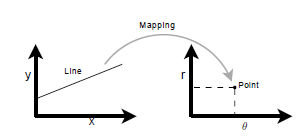
\includegraphics[scale=1]{rysunki/4_fig7}
	\caption{Odwzorowanie prostej w przestrzeni Hough’a}
\label{4_fig7}
\end{figure}
Posługując się parametrem $\theta$ określającym kąt pomiędzy wyznaczoną prostą a osią $x$ łatwo określić czy badane proste są do siebie równoległe. Aby wyznaczyć parametry prostej z równania \eqref{HOUGHTRANSFORM} zgodnie z \cite{houghTransform} należy każdemu punktowi tworzącemu prostą przypisać grupę punktów z przestrzeni Hough'a dla których wszystkie możliwe proste utworzone na ich podstawie zawierałyby badany punkt. Ostatecznie parametry prostej pochodzą z punktu, dla którego w przestrzeni Hough'a występuje największa gęstość powtarzających się punktów. Transformację przedstawia poniższy rysunek:
\begin{figure}[!h]
	\centering
	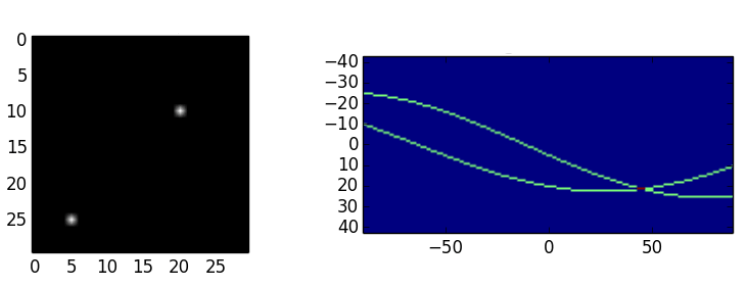
\includegraphics[scale=1]{rysunki/4_fig8}
	\caption{Transformacja dwóch punktów do dwóch krzywych w przestrzeni Hough'a. Źródło \cite{houghTransform}.}
\label{4_fig8}
\end{figure}
Dokładną analizę transformacji można znaleźć w \cite{houghTransform}.
Pojawiające się współczynniki $\alpha ,\beta ,\gamma $ w równaniu \eqref{SalientDistance} stanowią uprzednio definiowane wartości przypisujące procentowy wpływ poszczególnych członów na ostateczną wartość dopasowania $D(i,j)$. Według \cite{SalientStrucTexProp} najważniejszym dopasowaniem jest dopasowanie kolorów, następnie tekstur i krzywizn. Stąd należy przyjmować $\alpha >\beta >\gamma $ gdzie suma współczynników wynosi 1. W pracy zbadano powyższe rozwiązanie w ograniczeniu do wykorzystania członów $D_1\left(f^i_C,f^j_C\right)$ oraz $IP$. Człon $D_2\left(f^i_T,f^j_T\right)$ jest istotny w przypadku obrazów monochromatycznych o różnej teksturze. W przypadku obrazów kolorowych w większości przypadków linie granicy głównych struktur tworzone są poprzez gradienty kolorów. Zaletą metody jest stosowanie podzbiorów stanowiących źródło kopiowanych skrawków w nieznane części obrazu. W uproszczeniu można to przedstawić zgodnie z rysunkiem:
\begin{figure}[!h]
	\centering
	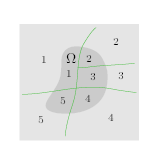
\includegraphics[scale=1]{rysunki/4_fig9}
	\caption{Grupowanie podzbiorów stanowiących źródło skrawków wykorzystywanych do syntezy podzbiorów nieznanego obszaru $\boldsymbol{\mathrm{\Omega }}$. źródło \cite{StructurePropagationManual}.}
\label{4_fig9}
\end{figure}
Pomimo automatycznej metody wykrywania i kontunuowania głównych struktur algorytm wymaga wielu operacji wykonywanych zdalnie przez użytkownika, takich jak stopień rozmycia wymagany do wprowadzenia w obrazie, wielkość kopiowanych skrawków $\psi $, czy też okien stanowiących podstawę do parowania danych struktur $f$. W przeciwieństwie do metod bazujących na rozwiązywaniu równań różniczkowych oraz metod bazujących na procesie dyfuzji proces wmalowywania opisany w aktualnym rozdziale pozbawiony jest wady w postaci rozmycia w odrestaurowanym obszarze. Jednym z problemów metody jest konieczność stosowania metody korekcji fotometrycznej zgodnie z \cite{StructurePropagationManual}, wygładzającej lokalne granice obrazu powstałe w wyniku syntezy skrawków obrazu $\psi $ w wyznaczanym obszarze $\mathrm{\Omega }$.
\chapter{Wmalowywanie struktury i tekstury obrazu.}
Metoda jednoczesnego wmalowywania struktur i tekstur stanowi połączenie wcześniej opisanych w pracy metod opartych o równania różniczkowe wyższego rzędu z metodami bazującymi na przykładowych źródłach kawałków obrazów stanowiących podstawę do wypełniania brakujących regionów. Pierwszy raz przedstawiona została przez Bertalmio i innych w 2003 roku w \cite{NavierStokesAndTexturePropagation}, a bardziej zaawansowany algorytm pojawia się w 2004 roku w [26]. Metoda w \cite{NavierStokesAndTexturePropagation} opiera się na wmalowywaniu struktury w oparciu o algorytm przedstawiony w \cite{bertalmio2000image} przy jednoczesnej propozycji prostej syntezy tekstury. 
\par
Niech obraz $I:R^2\to R,\ \ I\in L^2(R^2)$. Proces wypełniania brakującego regionu $\mathrm{\Omega }$ poprzedzony jest dekompozycją obrazu:
\begin{align}
I\left(i,j\right)=u\left(i,j\right)+v\left(i,j\right) 
\label{STRUCTURETEXTURE1}
\end{align}
uzyskaną na podstawie rozwiązania problemu minimalizacji energii:
\begin{align} 
{\mathop{\mathrm{min}}_{u} \Biggl\{E\left(u\right)=\int{\left|\mathrm{\nabla }u\right|+\lambda {\left|\left|v\right|\right|}^2_{L^2}}\Biggr\}\ }
\label{STRUCTURETEXTURE2}
\end{align}
gdzie: $\int{\left|\mathrm{\nabla }u\right|}$ stanowi funkcjonał z przestrzeni $BV(R^2)$ pozwalający usunąć z oryginalnego obrazu szum i powtarzające się w małej skali detale, przy jednoczesnym zachowaniu głównych cech oraz ostrych krawędzi, ${\left|\left|v\right|\right|}^2_{L^2}$ człon odpowiadający dokładności odwzorowania, $\lambda $ stanowi uprzednio definiowany parametr. Dla odpowiednio małych wartości $\lambda $ problem minimalizacji prowadzi do uzyskania jednorodnego komponentu $u$ reprezentującego odfiltrowany obraz oraz komponentu $v$ reprezentującego wahania w postaci szumu oraz tekstur. Zgodnie z dowodem Mayera w przypadku gdy pożądany jest wspomniany kształt funkcji $v$, można udowodnić jej  przynależność do przestrzeni Banacha oznaczanej $G$. W związku z tym (pomijając wyprowadzenia) problem minimalizacji można przedstawić w ostatecznej postaci minimalizacji energii:
\begin{align}
\begin{aligned} 
\mathop{\mathrm{min}}_{u,g_1,g_2} \Biggl\{E &= \int{\left|\mathrm{\nabla }u\right|+\lambda \int{{\left|I-u-{\partial }_xg_1-{\partial }_yg_2\right|}^2dxdy}} \\
&+ \mu {\left[\int{{\sqrt{g^2_1+g^2_2}}^pdxdy}\right]}^{\frac{1}{p}}\Biggr\}
\end{aligned}
\end{align}
gdzie:
\begin{align}
v=div\left(\mathop{g}\limits^{\rightharpoonup}\right),\ \mathop{g}\limits^{\rightharpoonup}=\left(g_1,g_2\right),\ g_1=-\frac{1}{2\lambda }\frac{u_x}{\left|\mathrm{\nabla }u\right|},\ g_2=-\frac{1}{2\lambda }\frac{u_y}{\left|\mathrm{\nabla }u\right|}\
\label{VG1G2}
\end{align}
oraz $p\to \mathrm{\infty }$. Stosując podstawowe równanie rachunku wariacyjnego postaci równania Eulera-Lagrange'a uzyskuje się odpowiadające mu postacie funkcji wykorzystywane do minimalizacji energii:
\begin{align}
u=I-u-{\partial }_xg_1-{\partial }_yg_2+\frac{1}{2\lambda }div\left(\frac{\mathrm{\nabla }u}{\left|\mathrm{\nabla }u\right|}\right)
\end{align}
\begin{align}
{\mu H\left(g_1,g_2\right)g}_1=2\lambda \left[\frac{\partial }{{\partial }_x}\left(u-I\right)+{\partial }^2_{xx}g_1+{\partial }^2_{xy}g_2\right]
\end{align}
\begin{align}
\mu H\left(g_1,g_2\right)g_2=2\lambda \left[\frac{\partial }{{\partial }_y}\left(u-I\right)+{\partial }^2_{xy}g_1+{\partial }^2_{yy}g_2\right]
\end{align}
gdzie $\mu$ stanowi uprzednio definiowany parametr dyskretyzacji, $H\left(g_1,g_2\right)$ opisuje się wzorem:
\begin{align}
H\left(g_1,g_2\right)={{{\left|\left|\sqrt{g^2_1+g^2_2}\right|\right|}_p}^{1-p}}{\left(\sqrt{g^2_1+g^2_2}\right)}^{p-2}
\end{align}
Zgodnie z \cite{vese2003modeling} w celach dyskretyzacji parametr $p$ przyjęto równy 1, ze względu na brak znaczących różnic wyniku w przypadku stosowania większych wartości. Wtedy:
\begin{align}
H\left(g_1,g_2\right)=\frac{1}{\sqrt{g^2_1+g^2_2}}
\end{align}
Formalnie, jednym z równań Eulera-Lagrange'a uzyskiwanym podczas minimalizacji wspomnianej energii $E$ jest:
\begin{align}
u=I+\frac{1}{2\lambda }div\left(\frac{\mathrm{\nabla }u}{\left|\mathrm{\nabla }u\right|}\right)
\end{align}
Stąd można wywnioskować:
\begin{align}
v=-\frac{1}{2\lambda }div\left(\frac{\mathrm{\nabla }u}{\left|\mathrm{\nabla }u\right|}\right)
\end{align}
Korzystając z zależności przedstawionych w \eqref{VG1G2} łatwo zauważyć $g^2_1+g^2_2=\frac{1}{2\lambda }$. Stąd:
\begin{align}
H\left(g_1,g_2\right)=\sqrt{2\lambda }
\end{align}
\begin{align}
u=I-u-{\partial }_xg_1-{\partial }_yg_2+\frac{1}{2\lambda }div\left(\frac{\mathrm{\nabla }u}{\left|\mathrm{\nabla }u\right|}\right)
\label{EU}
\end{align}
\begin{align}
\mu \sqrt{2\lambda }g_1=2\lambda \left[\frac{\partial }{{\partial }_x}\left(u-I\right)+{\partial }^2_{xx}g_1+{\partial }^2_{xy}g_2\right]
\label{EG1}
\end{align}
\begin{align}
\mu \sqrt{2\lambda }g_2=2\lambda \left[\frac{\partial }{{\partial }_y}\left(u-I\right)+{\partial }^2_{xy}g_1+{\partial }^2_{yy}g_2\right]
\label{EG2}
\end{align}
Jako wartości początkowe iteracyjnego algorytmu można przyjąć następujące przypuszczenie:
\begin{align}
u^0=f,\ g_1=-\frac{1}{2\lambda }\frac{f_{\mathrm{x}}}{\left|\mathrm{\nabla }f\right|},\ g_2=-\frac{1}{2\lambda }\frac{f_{\mathrm{y}}}{\left|\mathrm{\nabla }f\right|}
\end{align}
Następnie stosując zależności wyznaczania pochodnych \eqref{dfdx}, \eqref{dfdy}, \eqref{leftdfdx}, \eqref{leftdfdy} oraz poniższą metodę aproksymacji pochodnej drugiego stopnia:
\begin{align}
\begin{aligned} 
{\partial }_{xy}g_1\left(i,j\right) &\cong \frac{1}{2h^2}\ \bigg[2g_1\left(i,\ j\right)+g_1\left(i-1,\ j-1\right)+g_1\left(i+1,\ j+1\right)-g_1\left(i,\ j-1\right) \\ 
&-g_1\left(i-1,\ j\right)-g_1\left(i+1,\ j\right)-g_1\left(i,\ j+1\right)\bigg]
\end{aligned}
\end{align}
równania \eqref{EU}, \eqref{EG1} i \eqref{EG2} można przedstawić w następującej dyskretnej postaci:
\begin{align}
\begin{aligned}
u^{n+1}\left(i,j\right) &= \left[\frac{1}{\ 1\ +\ \left(\frac{1}{2\lambda h^2}\right)\cdot \left(c_1\left(i,j\right)+c_2\left(i,j\right)+c_3\left(i,j\right)+c_4\left(i,j\right)\right)\ }\right] \\ 
&\cdot \biggl[I\left(i,j\right)-\ \left(\frac{g^n_1\left(i+1,j\right)\cdot g^n_1\left(i-1,j\right)}{2h}\right)-\ \left(\frac{g^n_2\left(i,j+1\right)-g^n_2\left(i,j-1\right)}{2h}\right) \\ 
&+\ \left(\frac{1}{2\lambda h^2}\right)\cdot \Bigl[c_1\left(i,j\right)\cdot u^n\left(i+1,j\right)+c_2\left(i,j\right)\cdot u^n\left(i-1,j\right) \\
&+c_3\left(i,j\right)\cdot \lambda {\cdot u}^n\left(i,j+1\right)+c_4\left(i,j\right)\cdot u^n\left(i,j-1\right)\Bigr]\biggr]
\end{aligned}
\end{align}
\begin{align}
\begin{aligned}
g^{n+1}_1\left(i,j\right) &= \left[\frac{2\lambda }{\mu \sqrt{2\lambda }+\ 4\frac{\lambda }{2h}}\right]\cdot \Biggl[\frac{u^n\left(i+1,j\right)-u^n\left(i-1,j\right)}{2h}-\frac{I\left(i+1,j\right)-I\left(i-1,j\right)}{2h} \\
&+\frac{g_1\left(i+1,j\right)+g_1\left(i-1,j\right)}{h^2}\frac{1}{2h^2}\cdot \Bigl[2g^n_2\left(i,j\right)+\ g^n_2\left(i-1,j-1\right) \\ 
&+ g^n_2\left(i+1,j+1\right)
g^n_2\left(i,j-1\right)-\ g^n_2\left(i-1,j\right)+\ g^n_2\left(i+1,j\right) \\
&-g^n_2\left(i,j+1\right)\Bigr]\Biggr]
\end{aligned}
\end{align}
\begin{align}
\begin{aligned}
g^{n+1}_2\left(i,j\right) &=\left[\frac{2\lambda }{\mu \sqrt{2\lambda }\ +\ 4\frac{\lambda }{2h}}\right]\cdot \Biggl[\frac{u^n\left(i,j+1\right)-u^n\left(i,j-1\right)}{2h}-\frac{I\left(i,j+1\right)-I\left(i,j-1\right)}{2h} \\ 
&+\frac{g_2\left(i,j+1\right)+g_2\left(i,j-1\right)}{h^2}+\frac{1}{2h^2}\cdot \Bigl[2g^n_1\left(i,j\right)+\ g^n_1\left(i-1,j-1\right)+ g^n_1\left(i+1,j+1\right) \\
&-\ g^n_1\left(i,j-1\right)-\ g^n_1\left(i-1,j\right)+\ g^n_1\left(i+1,j\right)-\ g^n_1\left(i,j+1\right)\Bigr]\Biggr]
\end{aligned}
\end{align}
gdzie:
\begin{align}
\begin{aligned}
c^n_1\left(i,j\right)=\frac{1}{\sqrt{{\left(\frac{u^n\left(i+1,j\right)-u^n\left(i,j\right)}{h}\right)}^2+\ {\left(\frac{u^n\left(i,j+1\right)-u^n\left(i,j-1\right)}{2h}\right)}^2+\ \varepsilon }}
\end{aligned}
\end{align}
\begin{align}
\begin{aligned}
c^n_2\left(i,j\right)=\frac{1}{\sqrt{{\left(\frac{u^n\left(i,j\right)-u^n\left(i-1,j\right)}{h}\right)}^2+\ {\left(\frac{u^n\left(i-1,j+1\right)-u^n\left(i-1,j-1\right)}{2h}\right)}^2+\ \varepsilon }}
\end{aligned}
\end{align}
\begin{align}
\begin{aligned}
c^n_3\left(i,j\right)=\frac{1}{\sqrt{{\left(\frac{u^n\left(i+1,j\right)-u^n\left(i-1,j\right)}{2h}\right)}^2+\ {\left(\frac{u^n\left(i,j+1\right)-u^n\left(i,j\right)}{h}\right)}^2+\ \varepsilon }}\end{aligned}
\end{align}
\begin{align}
\begin{aligned}
c^n_4\left(i,j\right)=\frac{1}{\sqrt{{\left(\frac{u^n\left(i+1,j-1\right)-u^n\left(i-1,j-1\right)}{2h}\right)}^2+\ {\left(\frac{u^n\left(i,j\right)-u^n\left(i,j-1\right)}{h}\right)}^2+\ \varepsilon }}
\end{aligned}
\end{align}
W celu uniknięcia problemu dzielenia przez zero w powyższej dyskretyzacji wprowadzono parametr $\varepsilon \longrightarrow 0$. 
Po przeprowadzeniu powyższej segmentacji obrazu dla uzyskanych członów $u$ i $v$ można zastosować różne algorytmy wmalowywania braków. Zgodnie z ich charakterem najodpowiedniejszymi metodami wmalowywania struktur są metody oparte na równaniach różniczkowych, natomiast uzyskanie brakującej tekstury najlepiej wykonać metodą kopii kawałków obrazów z najlepszym dopasowaniem. W \cite{NavierStokesAndTexturePropagation} autorzy proponują następujący algorytm syntezy brakującej tekstury $\mathrm{\Omega }$:
\begin{figure}[!h]
	\centering
	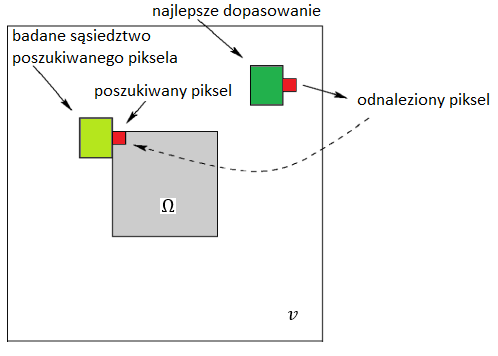
\includegraphics[scale=1]{rysunki/5_fig1}
	\caption{Prosty algorytm wmalowywania tekstury obrazu.}
	\label{5_fig1}
\end{figure}
Zgodnie z \autoref{5_fig1} dla każdego piksela znajdującego się na granicy $\mathrm{\Omega }$ tworzone jest okno stanowiące szablon wykorzystywany do odnalezienia najlepszego dopasowania z pośród całego obrazu $v$. W przypadku odnalezienia takiego dopasowania uzyskany piksel kopiowany jest w miejsce poszukiwanego piksela. Algorytm można wykonywać pobierając piksele z granicy w kolejności zgodnej ze wskazówkami zegara, postępując w głąb obszaru $\mathrm{\Omega }$, aż do wypełnienia wszystkich pikseli. Odnalezienie okna najlepszego dopasowania można wykonać analogicznie do metody wykorzystanej w publikacji Criminisi'ego, w oparciu o zależności \eqref{FROBDIST} oraz \eqref{FROBENIUS}. 

 W przypadku obrazów kolorowych pierwszym krokiem wykonania operacji wmalowywania jest transformacja do współrzędnych sferycznych zgodnie z zależnościami \eqref{TIone}, \eqref{TItwo} i \cite{TIthree} ze względu na ich lepsze właściwości. Następnie każda z trzech uzyskanych warstw jest rozbijana na własną teksturę i strukturę. W przypadku algorytmu dokonującego syntezy tekstury oddzielnie dla każdej z 3-ech segmentowanych warstw uzyskiwane wyniki charakteryzują się pojawiającymi się niespójnościami kolorów. Stąd w przypadku odrestaurowywania uzyskanych części $v$, zlokalizowanie piksela będącego najlepszym dopasowaniem aktualnie badanego, nieznanego piksela, odbywa się na podstawie pierwszej warstwy, a wszystkie 3 uzupełniane są analogicznie do obliczeń uzyskanych na podstawie pierwszej warstwy. Kroki algorytmu można przedstawić następująco:
\begin{enumerate}
\item
Przekształcenie warstw $R,G,B$ obrazu na współrzędne sferyczne $I_1,I_2,I_3$
\item
Wyznaczenie $u_1,v_1,\ u_2,v_2,u_3,v_3$ na podstawie $I_1,I_2,I_3$
\item
Wmalowanie nieznanych obszarów $\mathrm{\Omega }$ w warstwach $u_1,u_2,u_3$ metodą adaptacji równania Navier-Stokes'a
\item
Wmalowanie obszaru $\mathrm{\Omega }$ w $v_1,v_2,v_3$ na podstawie prostego algorytmu syntezy tekstury najlepszymi dopasowaniami uzyskanymi na podstawie warstwy $v_1$
\end{enumerate}

\chapter{Model wariacyjny z nielokalnym modelu wmalowywania}
Ostatnią z rozważanych metod będzie metoda zaproponowana przez autorów Fedorov, Facciolo i Arias w \cite{arias2011variational}. Autorzy w publikacji proponują optymalizację energii $\mathcal{E}(\varphi(x), u(\mathcal{O}))$ zależnej od dwóch niewiadomych:
\begin{itemize}
\item
nieznanego obszaru obrazu $u(\mathcal{O})$
\item
mapy podobieństwa będącej funkcją przypisującą każdemu puntowi z nieznanego obszaru jego odpowiednika z obszaru poza maską $\varphi(\hat{x})$
\end{itemize}
\begin{figure}[!h]
	\centering
	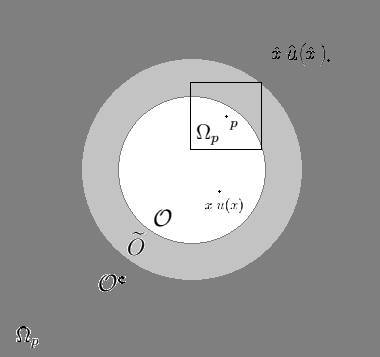
\includegraphics[scale=0.9]{rysunki/6_fig1}
	\caption{Określenie charakterystycznych obszarów obrazu.}
	\label{6_fig1}
\end{figure}
Zgodnie z \autoref{6_fig1} niech obraz stanowi przekształcenie $ u : {\Omega} \rightarrow R$, $\mathcal{O}$ oznacza obszar do uzupełnienia, $\mathcal{O}^c$ oryginalną część obrazu nie ulegającego modyfikacji, $\mathrm{\Omega }_p$ podzbiór pikseli scentrowanych względem  piksela $p \in \Omega$, gdzie $\Omega = \mathcal{O}^c + \mathcal{O}$, $\widetilde{\mathcal{O}} := \mathcal{O} + \mathrm{\Omega }_{ps}$, gdzie $\mathrm{\Omega }_{ps}$ oznacza sumę wszystkich zbiorów punktów $x \in \mathcal{O}$. Podobnie jak w \cite{arias2011variational} niech przekształcenie $u(x)$ jest zarezerwowane dla przestrzeni maski, a $\hat{u}(\hat{x})$ odpowiada przekształceniu w przestrzeni stałej obrazu $\widetilde{\mathcal{O}}$ ( $\hat{x} \in \mathcal{O}$). Mapowanie funkcji podobieństwa $\varphi(x)$ przedstawiono na \autoref{6_fig2}
\begin{figure}[!h]
	\centering
	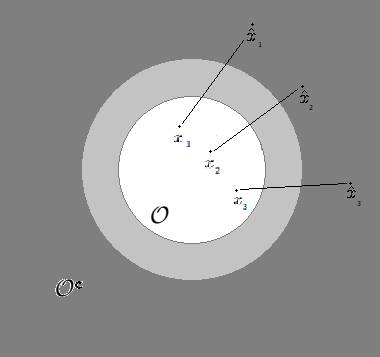
\includegraphics[scale=0.9]{rysunki/6_fig2}
	\caption{Funkcja podobieństwa $\varphi(\hat{x})$ : $x_1 = \varphi(\hat{x_1}), x_2 = \varphi(\hat{x_2}), x_3 = \varphi(\hat{x_3})$.}
	\label{6_fig2}
\end{figure}

$\mathcal{O}$

$\mathcal{E}$

$\widetilde O$

$\mathrm{\Omega }_p$

$x,u(x)$

$\hat{x}, \hat{u}(\hat{x})$

 



 





%-----------Koniec pracy magisterskiej-----------
\newpage
\bibliographystyle{unsrt}
\bibliography{bibliografia}

 
\tableofcontents
\clearpage
\pagestyle{empty}
\noindent Warszawa, dnia ...............
\vspace{5cm}
\begin{center}
\LARGE{Oświadczenie}
\end{center}
Ołwiadczam, że pracę magisterską pod tytułem: ,,Poprawa jakości obrazów cyfrowych poprzez metodę wmalowywania'', której promotorem jest dr Sławomir Skoneczny, wykonałem samodzielnie, co poświadczam własnoręcznym podpisem.
\vspace{2cm}
\begin{flushright}
...........................................
\end{flushright}

\end{document}